\documentclass[12pt,twoside,a4paper, openright]{report}
\usepackage{iisc_thesis}
\usepackage{etoolbox}
\AtBeginEnvironment{algorithm}{\setstretch{1}}
\AtBeginEnvironment{figure}{\setstretch{1}}
\AtBeginEnvironment{lstlisting}{\setstretch{1}}
\AtBeginEnvironment{SCfigure}{\setstretch{1}}
\AtBeginEnvironment{table}{\setstretch{1}}
\pagestyle{bfheadings}


\usepackage{hyperref}
\hypersetup{pdftex,colorlinks=true,allcolors=black}
\usepackage{hypcap}

\usepackage{graphicx}
\usepackage[caption=false]{subfig}
\usepackage{sidecap}
%\usepackage{subcaption}
\captionsetup[table]{font={stretch=1}}     %% change 1.2 as you like
\captionsetup[figure]{font={stretch=1}}    %% change 1.2 as you like
%\captionsetup{belowskip=0pt,aboveskip=2pt}
%\usepackage[outdir=./]{epstopdf}
\usepackage[cmex10]{amsmath}
\usepackage{enumitem}
\usepackage{leqno}
\newtheorem{mydef}{Definition}
\newtheorem{theorem}{Theorem}

\usepackage[ruled]{algorithm2e}
\SetAlgoLined
\SetKwFor{ForEach}{for each}{do}{endfor}
\SetKwInput{KwData}{Input}
\SetKwInput{KwResult}{Output}
\SetCommentSty{}

\usepackage[scaled]{beramono}
\usepackage[T1]{fontenc}
\usepackage[bitstream-charter]{mathdesign}
\usepackage{listings, multicol}
\lstset{ %
	basicstyle=\ttfamily,
	keywordstyle=\bfseries,
	language=Python,                     % choose the language of the code
	numbers=none,                   % where to put the line-numbers
	numberstyle=\footnotesize,      % the size of the fonts that are used for the line-numbers
	stepnumber=1,                   % the step between two line-numbers. If it is 1 each line will be numbered
	numbersep=3pt,                  % how far the line-numbers are from the code
	backgroundcolor=\color{white},  % choose the background color. You must add \usepackage{color}
	showspaces=false,               % show spaces adding particular underscores
	showstringspaces=false,         % underline spaces within strings
	showtabs=false,                 % show tabs within strings adding particular underscores
	frame=false,                    % adds a frame around the code
	tabsize=1,                      % sets default tabsize to 2 spaces
	captionpos=b,                   % sets the caption-position to bottom
	breaklines=true,                % sets automatic line breaking
	breakatwhitespace=false,        % sets if automatic breaks should only happen at whitespace
	escapeinside={(*}{*)},         % if you want to add a comment within your code
	framerule=0pt,
	morekeywords={Domain,Function,Interval,Reduction,Variable,
		Constant,Parameter,Kernel2D,Correlate,Min,Max,Sum,
		Image,Case,Default,Upsample,Downsample,Replicate,
		Reduce, UChar, Char, Float, Double, Int, UInt, 
		Short, UShort, Long, ULong, Condition, Stencil,
		TStencil, Grid, Interp, Restrict}
}

\makeatletter
\newcommand\footnoteref[1]{\protected@xdef\@thefnmark{\ref{#1}}\@footnotemark}
\makeatother

\usepackage{fancyhdr}

\fancyhf{}
\pagestyle{fancy}
\renewcommand{\chaptermark}[1]{\markboth{\thechapter.\ #1}{}}
\renewcommand{\sectionmark}[1]{\markright{\thesection.\ #1}{}}
% \renewcommand{\headrulewidth}{0.8pt}
\fancyhead[RO,LE]{\thepage}
\fancyhead[LO]{\rightmark}
\fancyhead[RE]{\leftmark}

\usepackage{varwidth}
\usepackage{multirow}
\usepackage{tabularx,booktabs, array}
\usepackage{url}

\usepackage{tikz}
\usepackage{tkz-graph}
\usetikzlibrary{shapes,arrows}
\usetikzlibrary{positioning, fit}
\usetikzlibrary{matrix}
\usetikzlibrary{calc}
\usepackage{pgfplots}
\graphicspath{{./images/}}
\pgfdeclarelayer{bg}    % declare background layer
\pgfdeclarelayer{nodelayer}
\pgfdeclarelayer{edgelayer}
\pgfsetlayers{bg,main,nodelayer,edgelayer}  % set the order of the layers (main is the standard layer)


% ADARSH MARCRO's
\newcommand{\cachename}{HAShCache}
\newcommand{\bypassname}{\textit{ByE}}
\newcommand{\prioname}{\textit{PrIS}}
\newcommand{\chaining}{\textit{Chaining}}

\newcommand{\blankpage}{
	\newpage
	\thispagestyle{empty}
	\mbox{}
	\newpage
}


\begin{document}

\begin{frontmatter}
\title{Heterogeneity Aware Shared DRAM Cache for \\ Integrated Heterogeneous Architectures}
\author{Adarsh Patil}
\dept{Department of Computer Science and Automation}
\enggfaculty
%\degreein{Computer Science and Engineering}
\mscengg
\iisclogotrue % Default is false
\figurespagefalse %default is true
\tablespagetrue %default is false
\maketitle

\vspace*{\fill}
\vspace{10em}
\begin{center}
	\Large\bf \textcopyright \ Adarsh Patil\\
	\Large\bf July 2017\\
	\Large\bf All rights reserved
\end{center}
\vspace*{\fill}
\pagenumbering{gobble}
\thispagestyle{empty}


\begin{dedication}
\newpage
\vspace*{\fill}
\begin{center}
	DEDICATED TO \\
	\Large\it My Parents  \\
	\Large\it and Kumudha
\end{center}
\vspace*{\fill}
\thispagestyle{empty}
\newpage
\thispagestyle{empty}
\end{dedication}


\acknowledgements
\pagenumbering{roman}
My experience at IISc has been nothing short of incredible and several thanks are in order.
\par First and foremost, I would like to express my deeprest gratidude to my research advisor Prof. R. Govindarajan for being a supportive mentor and guide. He has been patient with me and has encouraged, taught and motivated me to think clearly and critically. His humbleness, knowledge and relentless work ethic will always be a constant source of inspiration to me.
\par I owe a deep sense of gratitude to everyone who have made my stay at IISc comfortable. A big thanks to the department chairman Professor Jayant Haritsa and Professor Uday Reddy whose backing and ecouragement towards student system admin activities and their endorsement for compute infrastructure make the department well equipped to perform research. I am grateful to the staff at CSA office and the system admins Jagdish and Pushparaj who work tirelessly to keep the department and compute resources running. Thanks are also due for the funding sources - MHRD and AMD for supporting me financially to take care of my day-to-day expenses. I have greatly enjoyed courses by Professor Matthew Jacob and Professor Jayant Haritsa and their refreshing ways of course instruction.
\par I also want to acknowledge everyone in the HPC lab - Jayvant, Shilpa, Abhinav, Nagendra and Arth for providing a friendly and constructive atmosphere in the lab and for their useful feedback and insightful comments on my work. It was great sharing lab discussions and deliberating over problems and findings. My thanks also go out to my wonderful friends at IISc - Arvind, Vinay, Sridhar, Srinidhi, Anirudh, Pallavi, Sathya, Divya and several others who are not mentioned here. It was a pleasure sharing the many meals, dinner and ice cream outings and the lively banter in the mess. You always made sure there was never a dull moment and made my stint here truly memorable.
\par I would also like to thank Vikram, Archana, Aditya, Divyanshu and the members of IISc Running Club for organizing wondeful running events on campus and giving me a chance to represent the institute at the 12 hour relay run. It was wonderful being running buddies with all of you. I will always fondly remember my morning runs at this wondeful and serene campus which provided a harmonious evironment throughout the year and has always reinvigorated and rejuvenated my spirits in silence.
\par I must express my profound gratitude to my parents for their unconditional support for all my decisions, their counsel and lending me a sympathetic ear when I needed it. Finally, I thank Kumudha who has always been there for me, be it for technical advice or moral support. Her unyielding love has been my source of strength. My gratitude also goes to my parents-in-law who have been so supportive of us.\\
\\
\par Thank you very much, everyone!


\publications
\begin{enumerate}
	\item A. Patil, R. Govindarajan. \cachename: Heterogeneity Aware Shared DRAM Cache for Integrated Heterogeneous Systems. Submitted to ACM \textit{Transactions on Architecture and Code Optimization (TACO)}
\end{enumerate}



\begin{abstract}
\par Integrated Heterogeneous System (IHS) processors pack throughput-oriented GPGPUs alongside latency-oriented CPUs on the same die sharing certain resources, e.g., shared last level cache, network-on-chip (NoC), and the main memory. They also share virtual and physical address spaces and unify the memory hierarchy. The IHS architecture allows for easier programmability, data management and efficiency. However, the significant disparity in the demands for memory and other shared resources between the GPU cores and CPU cores poses significant problems in exploiting the full potential of this architecture.
\par In this work, we propose adding a large capacity stacked DRAM, used as a shared last level cache, for the IHS processors. The reduced latency of access and large bandwidth provided by the DRAM cache can help improve performance respectively of CPU and GPGPU while the large capacity can help contain the working set of the IHS workloads. However, adding the DRAM cache naively, leaves significant performance on the table due to the disparate demands from CPU and GPU cores for DRAM cache and memory accesses. 
In particular, the imbalance can significantly reduce the performance benefits that the CPU cores would have otherwise enjoyed with the introduction of the DRAM cache. This necessities a heterogeneity-aware management of this shared resource for improved performance. To address this, in this thesis, we propose three simple techniques to enhance the performance of CPU application while ensuring very little or no performance impact to the GPU. Specifically, we propose (i) \prioname, a prioritization scheme for scheduling CPU
requests at the DRAM cache controller, (ii) \bypassname, a selective and temporal bypassing scheme for CPU requests at the DRAM cache and (iii) \chaining, an occupancy controlling mechanism for GPU lines in the DRAM cache through pseudo-associativity. The resulting cache, \cachename, is heterogeneity-aware and can adapt dynamically to address the inherent disparity of demands in an IHS architecture with simple light weight schemes. 
\par We enhance the gem5-gpu simulator to model an IHS architecture with stacked DRAM as a cache, coherent GPU L2 cache and CPU caches and a shared unified physical memory. Using this setup we perform detailed experimental evaluation of the proposed \cachename\ and demonstrate an average system performance (combined performance of CPU  and GPU cores) improvement of 41\% over a naive DRAM cache and over 100\% improvement over a baseline system with no stacked DRAM cache.

\end{abstract}

\makecontents

	
\cleardoublepage
\addcontentsline{toc}{chapter}{\listfigurename}
\listoffigures

\newpage
\addcontentsline{toc}{chapter}{List of Algorithms}
\listofalgorithms
\newpage
\thispagestyle{empty}
\cleardoublepage


\end{frontmatter}

\usetikzlibrary{shapes,arrows}
\usetikzlibrary{backgrounds}
\usetikzlibrary{matrix, positioning, fit}
\usetikzlibrary{patterns}
\definecolor{forestgreen}{rgb}{0.0, 0.5, 0.0}

\tikzstyle{smallcircle} =[fill=black!100, text=white, circle, inner sep=1pt, minimum size=0.1em]
\tikzstyle{ourcircle} = [draw, semicircle, inner sep=0pt,minimum size=2pt]
\tikzstyle{dullblock} = [draw, fill=black!20, circle, minimum height=2em, minimum width=2em]
\tikzstyle{block} = [draw=black, rounded corners, thick, line width=0.3mm, rectangle, minimum height=10em, minimum width=7em]
\tikzstyle{blocksmall} = [draw=black, thick, line width=0.5mm, rectangle, minimum height=6em, minimum width=3em, fill=white]
\tikzstyle{group} = [draw=black, line width=0.3mm, rectangle, minimum height=2em, minimum width=2em]
\tikzstyle{textblock} = [draw, fill=black!20, rectangle, rounded corners]
\tikzstyle{rectblock} = [draw, rectangle, minimum height=1.3em]
\tikzstyle{plain} = []
\tikzstyle{decisionblock} = [draw, diamond, fill=black!20]
\tikzstyle{input} = [draw, thick, fill=blue!20, circle, minimum size=1pt]
\tikzstyle{output} = [draw, fill=blue!20, circle, minimum size=1pt]
\tikzstyle{pinstyle} = [pin edge={to-,thin,black}]
\tikzset{toprule/.style={%
        execute at end cell={%
            \draw [line cap=rect,#1] (\tikzmatrixname-\the\pgfmatrixcurrentrow-\the\pgfmatrixcurrentcolumn.north west) -- (\tikzmatrixname-\the\pgfmatrixcurrentrow-\the\pgfmatrixcurrentcolumn.north east);%
        }
    },
    bottomrule/.style={%
        execute at end cell={%
            \draw [line cap=rect,#1] (\tikzmatrixname-\the\pgfmatrixcurrentrow-\the\pgfmatrixcurrentcolumn.south west) -- (\tikzmatrixname-\the\pgfmatrixcurrentrow-\the\pgfmatrixcurrentcolumn.south east);%
        }
    }
}


\newcommand{\bloom}[0]{
    \begin{tikzpicture}[auto, >=latex']
        % Blocks
        \node [textblock, thick, minimum height=5em] (bye){\begin{varwidth}{4cm} \centering{\footnotesize{B\\y\\E\\}} \end{varwidth}};
        \node [textblock, thick, minimum width=6em, minimum height=4em, right = 1.5cm of bye, yshift=2.2cm] (dramcache){\begin{varwidth}{4cm} \centering{\footnotesize{DRAM\\Cache}} \end{varwidth}};
        \node [textblock, thick, left = 0.01cm of dramcache, xshift=1.5em] (pred){\begin{varwidth}{4cm} \centering{\tiny{P\\R\\E\\D\\}} \end{varwidth}};
        \node [textblock, thick, left = 0.01cm of dramcache] (queue){\begin{varwidth}{4cm} \centering{\footnotesize{I I I I}} \end{varwidth}};
        \node [textblock, thick, minimum width=4em, right = 5cm of bye, minimum height=7em, yshift=-0.5cm] (dram){\begin{varwidth}{4cm} \centering{\footnotesize{Off-Chip\\DRAM\\Memory}} \end{varwidth}};

        % Arrows
        \draw [<-,very thick] (bye.west) to [out=180,in=0] ++(-0.6,0);
        \draw [->, very thick] (dramcache.east) to [out=0,in=180] ++(2.1,0) to (dram.north);
        \draw [->, very thick] ([yshift=1em]dramcache.east) to [out=0,in=180] ++(3.5,0);
        \draw [->, very thick] (dram.east) to [out=0,in=180] ++(1.1,0);
        \draw [<-, very thick] (queue.south) to ++(0.12,-0.85) to [out=180,in=0] ++(-1.35,0) to (bye.north);
        \draw [->, very thick] (dramcache.south) to [out=-90,in=90] ++(0,-0.8) to [out=180,in=0] ++(-2.6,0);
        \draw [->, very thick] ([yshift=2.5em] dram.west) to ++(-1.6,0) to ([xshift=2.3em] dramcache.south);
        \draw [<->, very thick] (bye.south) to [out=-90,in=90] ++(0,-0.5) to [out=0,in=180] ++(5.25,0);
        \draw [->, very thick] (bye.east) to [out=0,in=180] ++(5,0);
        \draw [<-, very thick] (queue.west) to ++(-0.45,0.45) to ++(-1,0);
        \draw [<-, very thick] (queue.west) to ++(-0.45,-0.45) to ++(-1,0);
        \draw [-, very thick, xshift=3.2cm] (0,1.5) to (0,0.16);
        \draw [-, very thick, xshift=3.2cm, right=90, looseness=3] (-0.07,0.067) to (0,-0.15);
        \draw [->, very thick, xshift=3.2cm] (0.01,-0.13) to (0,-1.4);
        \draw [->, dashed] (pred.east) to [out=0,in=180] ++(1.65,0);

        % labels
        \node [plain, left=0.01cm of bye, minimum height=1em, minimum width=1em] (cpurd) {\begin{varwidth}{4cm}\scriptsize{CPU\\ \\Rd}\end{varwidth}};
        \node [plain, above=1.4cm of dram, minimum height=1em, minimum width=1em, xshift=-2.8em, yshift=-1.8em] (cachemiss) {\begin{varwidth}{4cm}\scriptsize{Cache Miss/\\Pred Off-chip acess}\end{varwidth}};
        \node [plain, left=1.2cm of dram, minimum height=1em, minimum width=1em, yshift=-3em] (dirtyevict) {\begin{varwidth}{4cm}\scriptsize{Dirty Eviction}\end{varwidth}};
        \node [plain, left=0.4cm of dramcache, minimum height=1em, minimum width=1em, yshift=-1.44em, xshift=-2em] (WrReq) {\begin{varwidth}{4cm}\scriptsize{CPU Wr\\ Req}\end{varwidth}};
        \node [plain, left=0.3cm of dramcache, minimum height=1em, minimum width=1em, yshift=1.2em, xshift=-1.8em] (GpuReq) {\begin{varwidth}{4cm}\scriptsize{GPU Rd/Wr \\Req}\end{varwidth}};
        \node [plain, right=0.2cm of bye, minimum height=1em, minimum width=1em, yshift=1.25cm, xshift=-0.5cm] (maydir) {\begin{varwidth}{4cm}\scriptsize{Maybe Dirty}\end{varwidth}};
        \node [plain, right=0.2cm of bye, minimum height=1em, minimum width=1em, yshift=0.1cm, xshift=1cm] (notdir) {\begin{varwidth}{4cm}\scriptsize{Not Dirty}\end{varwidth}};
        \node [plain, below=0.15cm of maydir, minimum height=1em, minimum width=1em, xshift=1cm, yshift=0.2cm] (wrhit) {\begin{varwidth}{4cm}\scriptsize{Write Hit}\end{varwidth}};
        \node [plain, left=0.01cm of dram, minimum height=1em, minimum width=1em, yshift=3em] (fill) {\begin{varwidth}{4cm}\scriptsize{GPU Fill}\end{varwidth}};
        \node [plain, above=0.01pt of queue, minimum height=1em, minimum width=1em, yshift=-0.3em] (reqq) {\begin{varwidth}{4cm}\scriptsize{Req Q}\end{varwidth}};
        \node [plain, right=0.01pt of dram, minimum height=1em, minimum width=1em] (cpubypass) {\begin{varwidth}{4cm}\scriptsize{CPU Resp\\Bypass}\end{varwidth}};
        \node [plain, right=1.5cm of dramcache, minimum height=1em, minimum width=1em, yshift=1em] (datadram) {\begin{varwidth}{4cm}\scriptsize{Resp from\\ DRAM Cache}\end{varwidth}};


    \end{tikzpicture}

}

\newcommand{\chainaccess}[0]{
    \begin{tikzpicture}[auto, >=latex']
        % We start by placing the blocks
        \node [textblock, thick, minimum width=6em] (act){\begin{varwidth}{4cm} \centering{\footnotesize{DRAM $\$$ \\Row Act.}} \end{varwidth}};
        \node [textblock, thick, right = 0.5cm of act, minimum width=4em] (burst) {\begin{varwidth}{4cm} \centering{\footnotesize{TAD \\Burst}} \end{varwidth}};
        \node [decisionblock, thick, right = 0.5cm of burst] (tagmatch) {\begin{varwidth}{4cm} \centering{\scriptsize{Tag\\Match}} \end{varwidth}};
        \node [textblock, thick, below = 0.5cm of tagmatch] (chaintable) {\begin{varwidth}{4cm} \centering{\footnotesize{Chain\\Offset}} \end{varwidth}};
        \node [decisionblock, thick, right = 1.8cm of tagmatch.south] (clean) {\begin{varwidth}{4cm} \centering{\scriptsize{Clean?}} \end{varwidth}};
        \node [decisionblock, thick, right = 2.1cm of tagmatch, yshift=1.5em] (pamreturn) {\begin{varwidth}{4cm} \centering{\scriptsize{PAM \\return?}} \end{varwidth}};
        \node [textblock, thick, right = 1.5cm of pamreturn.south, minimum width=4em, yshift=-1em] (chaintad) {\begin{varwidth}{4cm} \centering{\footnotesize{Chain\\TAD}} \end{varwidth}};
        \node [decisionblock, thick, right = 0.5cm of chaintad] (chainmatch) {\begin{varwidth}{4cm} \centering{\scriptsize{Tag\\Match}} \end{varwidth}};
        \node [textblock, thick, right = 0.5cm of chainmatch, minimum height=7em, yshift=1.5em] (mem) {\begin{varwidth}{4cm} \centering{\footnotesize{Off-chip\\DRAM\\Memory}} \end{varwidth}};

        % Arrows
        \draw [->,very thick] (act) -- (burst);
        \draw [->,very thick, red] (chaintable.east) -- (clean);
        \draw [->,very thick] (burst) -- (tagmatch);
        \draw [->,very thick] (tagmatch.south) -- (chaintable.north);
        \draw [->,very thick] (tagmatch.east) to [out=0,in=180] ++(0.5,0) to [out=90,in=-90] ++(0,1.5);
        \draw [->,very thick, red] (clean.north) to [out=90,in=-90] ++(0,0.65) to (pamreturn.west);
        \draw [->,very thick, red] (pamreturn.south)to [out=-90,in=90] ++(0,-0.3) to [out=0,in=180] ++(1.5,0);
        \draw [->,very thick, red] (pamreturn.east) to [out=0,in=180] ++(0.5,0) to [out=90,in=-90] ++(0,0.5);
        \draw [->,very thick, red] (clean.east) to [out=0,in=180] ++(2.2,0);
%        \draw [->,very thick] (chaintable.south) to [out=0,in=180] ++(9.65,0) to (mem.south);
        \draw [->,very thick] (chainmatch.east) to [out=0,in=180] ++(0.6,0);
        \draw [->,very thick] (chaintad.east) -- (chainmatch);
        \draw [->,very thick] (chainmatch.north) to [out=90,in=-90] ++(0,1);
        \draw [->,very thick] (chaintable.east) to [out=0,in=180] ++(5.7,0) to (chaintad.south);
        \draw [->,very thick] (chaintable.east) to [out=0,in=180] ++(0.3,-0.4) to [out=0,in=180] ++(9.65,0) to (mem.south);

        % Groups
        \node [blocksmall, draw=white, above = 1cm of clean, minimum height=1em, minimum width=0.2em, xshift=-0.7em, yshift=0.4em] (lblcpu){\textbf{CPU}};
        \node[group, dashed, inner sep = 1pt, line width=0.3mm, draw=red, fit=(clean)(pamreturn)] (cpugroup) {};

        % Labels
        \node [plain, right=0.01em of tagmatch, minimum height=1em, minimum width=1em, yshift=1em, xshift=-0.5em] (lbl1) {\footnotesize{\emph{Hit}}};
        \node [plain, below=0.01em of tagmatch, minimum height=1em, minimum width=1em, xshift=-1.2em] (lbl2) {\footnotesize{\emph{Miss}}};
        \node [plain, below=0.52cm of tagmatch, minimum height=1em, minimum width=1em, xshift=4em] (lbl3) {\footnotesize{\emph{Yes}}};
        \node [plain, below=0.1cm of lbl3, minimum height=1em, minimum width=1em, yshift=0.2em] (lbl4) {\footnotesize{\emph{No}}};
        \node [plain, above=0.01cm of lbl3, minimum height=1em, minimum width=1em, red] (lb15) {\footnotesize{\emph{Yes}}};
        \node [plain, right=0.01em of chainmatch, minimum height=1em, minimum width=1em, yshift=-0.5em, xshift=-0.65em] (lbl5) {\footnotesize{\emph{Miss}}};
        \node [plain, above=3em of lbl5, minimum height=1em, minimum width=1em, yshift=-0.5em, xshift=-2em] (lbl8) {\footnotesize{\emph{Hit}}};
        \node [plain, right=0.01em of clean, minimum height=1em, minimum width=1em, yshift=-0.5em, red] (lbl6) {\footnotesize{\emph{No}}};
        \node [plain, right=2.5em of lbl6, minimum height=1em, minimum width=1em, yshift=1.5em, xshift=-1.5em, red] (lbl7) {\footnotesize{\emph{No}}};
        \node [plain, above=1.8em of clean, minimum height=1em, minimum width=1em, xshift=-0.1em, red] (lbl9) {\footnotesize{\emph{Yes}}};
        \node [plain, above=1.8em of chaintad, minimum height=1em, minimum width=1em, yshift=0.5em, xshift=-1.5em, red] (lbl10) {\footnotesize{\emph{Yes}}};
        \node [plain, above=0.3em of lbl10, minimum height=1em, minimum width=1em] (lbl11) {\footnotesize{\emph{Return Data}}};
        \node [plain, left=9.7em of lbl11, minimum height=1em, minimum width=1em] (lbl12) {\footnotesize{\emph{Return Data}}};
        \node [plain,right =2.5em of lbl11, minimum height=1em, minimum width=1em] (lbl13) {\footnotesize{\emph{Return Data}}};

        % Row Buffer
        \node [rectblock, thick, above = 2.4cm of act, minimum width=6.5em] (data) {\begin{varwidth}{4cm} \centering{\footnotesize{DATA}} \end{varwidth}};
        \node [rectblock, thick, right = 0cm of data, minimum width=4em] (tag) {\begin{varwidth}{4cm} \centering{\footnotesize{TAG}} \end{varwidth}};
        \node [rectblock, thick, right = 0cm of tag, minimum width=1pt] (isgpu) {\begin{varwidth}{4cm} \centering{\scriptsize{}} \end{varwidth}};
        \node [rectblock, thick, right = 0cm of isgpu] (chain) {\begin{varwidth}{4cm} \centering{\scriptsize{}} \end{varwidth}};
        \node [rectblock, thick, right = 0cm of chain] (reversechain) {\begin{varwidth}{4cm} \centering{\scriptsize{}} \end{varwidth}};
        \node [rectblock, thick, right = 0cm of reversechain, minimum width=1pt] (chaindirty) {\begin{varwidth}{4cm} \centering{\scriptsize{}} \end{varwidth}};
        \node [rectblock, thick, right = 0cm of chaindirty, minimum width=9em] (tad2) {\begin{varwidth}{4cm} \centering{\scriptsize{\textbf{TAD 2}}} \end{varwidth}};
        \node [rectblock, thick, right = 0cm of tad2, minimum width=8em] (row) {\begin{varwidth}{4cm} \centering{\textbf{...}} \end{varwidth}};
        \node [rectblock, thick, right = 0cm of row, minimum width=9em] (tad15) {\begin{varwidth}{4cm} \centering{\scriptsize{\textbf{TAD 15}}} \end{varwidth}};
        \node [rectblock, thick, right = 0cm of tad15, minimum width=1.2em] (cg) {\begin{varwidth}{4cm} \centering{} \end{varwidth}};
        \node [rectblock, thick, right = 0cm of cg, minimum width=2em, pattern=north west lines] (dc) {\begin{varwidth}{4cm} \centering{} \end{varwidth}};
        \draw [decorate,decoration={brace,amplitude=5pt},yshift=8.7em, xshift=-2.8em] (0,0.3) -- (4.6,0.3) node [black,midway,yshift=0.5em] {\footnotesize \textbf{TAD 1} ($128B + 8B$)};
        \draw [decorate,decoration={brace,amplitude=5pt},yshift=8.7em, xshift=3.2em] (11.75,0.3) -- (12.9,0.3) node [black,midway,yshift=0.5em] {\footnotesize $8B$ unused};

        \node [plain, below=0.4cm of chain, minimum height=1em, minimum width=1em, xshift=-1.6em] (lbl31){\begin{varwidth}{4cm} \centering{\footnotesize{2bit Chain}} \end{varwidth}};
        \node [plain, below=0.7cm of reversechain, minimum height=1em, minimum width=1em, xshift=1em] (lbl32) {\begin{varwidth}{4cm} \centering{\footnotesize{2bit Reverse Chain}} \end{varwidth}};
        \node [plain, below=0.2cm of chaindirty, minimum height=1em, minimum width=1em, xshift=2.4em] (lbl33) {\begin{varwidth}{4cm} \centering{\footnotesize{1bit Chain Dirty}} \end{varwidth}};
        \node [plain, below=0.1cm of cg, minimum height=1em, minimum width=1em, xshift=1em] (lbl34) {\begin{varwidth}{4cm} \centering{\footnotesize{CPU/GPU bitvector(15 bits)}} \end{varwidth}};
        \node [plain, below=0.1cm of isgpu, minimum height=1em, minimum width=1em, xshift=-1.8em] (lbl35) {\begin{varwidth}{4cm} \centering{\footnotesize{CPU/GPU}} \end{varwidth}};

        \draw [<-] (chain.south) to [out=-90,in=90] ++(0,-0.5);
        \draw [<-] (reversechain.south) to [out=-90,in=90] ++(0,-0.8);
        \draw [<-] (chaindirty.south) to [out=-90,in=90] ++(0,-0.3);
        \draw [<-] (cg.south) to [out=-90,in=90] ++(0,-0.2);
        \draw [<-] (isgpu.south) to [out=-90,in=90] ++(0,-0.2);

    \end{tikzpicture}
}

\newcommand{\hsacpu}[0]{
    \begin{tikzpicture}[auto, >=latex']
        %CPU
        \node [blocksmall, minimum height=1em, minimum width=1em] (cpu1) {\begin{varwidth}{4cm}\centering{CPU\\ Core 1} \end{varwidth}};
        \node [blocksmall, above = 0.1cm of cpu1, minimum height=1em, minimum width=1em] (l11){\begin{varwidth}{4cm} \centering{L1} \end{varwidth}};
        
        %\node [blocksmall, right = 0.1cm of cpu1, minimum height=1em, minimum width=1em] (cpu2) {\begin{varwidth}{4cm} \centering{CPU\\ Core 2} \end{varwidth}};
        %\node [blocksmall, above = 0.1cm of cpu2, minimum height=1em, minimum width=1em] (l12){\begin{varwidth}{4cm} \centering{L1} \end{varwidth}};
        
        \node [smallcircle, right=0.15cm of cpu1] (dot1) {};
        \node [smallcircle, right=0.05cm of dot1] (dot2) {};
        \node [smallcircle, right=0.05cm of dot2] (dot3) {};
        
        %\node [blocksmall, right = 0.1cm of cpu2, minimum height=1em] (cpu3){\begin{varwidth}{4cm} \centering{CPU\\ Core 3} \end{varwidth}};
        %\node [blocksmall, above = 0.1cm of cpu3, minimum height=1em] (l13){\begin{varwidth}{4cm} \centering{L1} \end{varwidth}};
        
        \node [blocksmall, right = 0.15cm of dot3, minimum height=1em, minimum width=1em] (cpu4){\begin{varwidth}{4cm} \centering{CPU\\ Core N} \end{varwidth}};
        \node [blocksmall, above = 0.1cm of cpu4, minimum height=1em, minimum width=1em] (l14){\begin{varwidth}{4cm} \centering{L1} \end{varwidth}};
        \node [blocksmall, above = 2.01cm of dot3, minimum height=3em, minimum width=6em] (l24){\begin{varwidth}{4cm} \centering{L2} \end{varwidth}};
        
       % \begin{scope}[on background layer]
            %\node[group, inner sep = 3pt, line width=0.3mm, draw=red, yshift=1em, fit=(cpu1)(cpu2)(cpu3)(cpu4)(l11)(l12)(l13)(l14)(l24)] (grpcpu) {};
       % \end{scope}
        
        
        %GPU
        \node [blocksmall, right = 0.6cm of cpu4, minimum height=1.5em, minimum width=1em] (sm1) {CU};
        \node [blocksmall, above = 0.1cm of sm1, minimum height=1pt, minimum width=1em] (sm1l1) {\scriptsize{L1}};
        \node [blocksmall, right = 0.15cm of sm1, minimum height=1.5em, minimum width=1em] (sm2) {CU};
        \node [blocksmall, above = 0.1cm of sm2, minimum height=1em, minimum width=1em] (sm2l1) {\scriptsize{L1}};
        \node [blocksmall, right = 0.15cm of sm2, minimum height=1.5em, minimum width=1em] (sm3) {CU};
        \node [blocksmall, above = 0.1cm of sm3, minimum height=1em, minimum width=1em] (sm3l1) {\scriptsize{L1}};
        \node [blocksmall, right = 0.15cm of sm3, minimum height=1.5em, minimum width=1em] (sm4) {CU};
        \node [blocksmall, above = 0.1cm of sm4, minimum height=1em, minimum width=1em] (sm4l1) {\scriptsize{L1}};
        \node [blocksmall, above = 2.3cm of sm1, minimum height=1.5em, minimum width=1em] (sm5) {CU};
        \node [blocksmall, below = 0.1cm of sm5, minimum height=1em, minimum width=1em] (sm5l1) {\scriptsize{L1}};
        \node [blocksmall, right = 0.15cm of sm5, minimum height=1.5em, minimum width=1em] (sm6) {CU};
        \node [blocksmall, below = 0.1cm of sm6, minimum height=1em, minimum width=1em] (sm6l1) {\scriptsize{L1}};
        \node [blocksmall, right = 0.15cm of sm6, minimum height=1.5em, minimum width=1em] (sm7) {CU};
        \node [blocksmall, below = 0.1cm of sm7, minimum height=1em, minimum width=1em] (sm7l1) {\scriptsize{L1}};
        \node [blocksmall, right = 0.15cm of sm7, minimum height=1.5em, minimum width=1em] (sm8) {CU};
        \node [blocksmall, below = 0.1cm of sm8, minimum height=1em, minimum width=1em] (sm8l1) {\scriptsize{L1}};  
        
        \node [blocksmall, minimum height=1.1em, minimum width=6em] at (5.6,1.45)
        (l2gpu) {\begin{varwidth}{4cm} \centering{\small{Coherent GPU \\L2}}\end{varwidth}};
        
         %\begin{scope}[on background layer]
            \node[group, inner sep = 3pt, line width=0.3mm, draw=red, fit=(sm1)(sm1l1)(sm2)(sm2l1)(sm3)(sm3l1)(sm4)(sm4l1)(sm5)(sm5l1)(sm6)(sm6l1)(sm7)(sm7l1)(sm8)(sm8l1)(l2gpu)] (grpgpu) {};
         %\end{scope}                        
        
        
        %Interconnect
        \node [blocksmall, minimum height=1.5em, minimum width=10.7em] at (1.5,1.5)
        (interconnect) {Cache Coherent Interconnect};
                
        %Connections to interconnect
        \draw [-,very thick] (l11.north) to ++(0, 0.15); 
        \draw [-, very thick] (l24.south) to ++(0, -0.3);
        \draw [-, very thick] (l2gpu.west) to ++(-0.82,0);
        \draw [-, very thick] (l14.north) to ++(0, 0.15);
        %\draw [-, very thick] (l13.north) to ++(0, 0.15);
        %\draw [-, very thick] (l12.north) to ++(0, 0.15);
        
        % Memory Controller
        \node [blocksmall, minimum height=1em, minimum width=9em, below=0.1cm of cpu4, xshift=-2em] (mc1){\begin{varwidth}{4cm} \centering{Memory Controller} \end{varwidth}};
        \node [blocksmall, minimum height=1em, minimum width=9em, right=0.05cm of mc1] (mc2){\begin{varwidth}{4cm} \centering{Memory Controller} \end{varwidth}};  
        
        %\draw [-, very thick] (-0.78,-0.6) to (-0.78, 1.5) to (interconnect.west);
        \draw [-, very thick] (2.8,-0.6) to (2.8, 1.25);
        \draw [-, very thick] (3.07,-0.6) to (3.07, 1.25);
        
        %Chip
        \begin{scope}[on background layer]
             \node[group, inner sep = 4pt, line width=0.6mm, fill=cyan!70, fit=(cpu1)(cpu4)(l11)(l14)(l24)(interconnect)(mc1)(mc2)(grpgpu)] (grpchip) {};
        \end{scope}

        % GPU L1 to L2 connections
        \draw [-,very thick] (sm1l1.north east) -- (l2gpu);
        \draw [-,very thick] (sm2l1.north) -- (l2gpu);
        \draw [-,very thick] (sm3l1.north) -- (l2gpu);
        \draw [-,very thick] (sm4l1.north) -- (l2gpu);
        \draw [-,very thick] (sm5l1.south east) -- (l2gpu);
        \draw [-,very thick] (sm6l1.south) -- (l2gpu);
        \draw [-,very thick] (sm7l1.south) -- (l2gpu);                
        \draw [-,very thick] (sm8l1.south) -- (l2gpu);

        % Off package Region
        \node [blocksmall, below = 3em of mc1, draw=black!30, fill=black!30, minimum height=0.5em, minimum width=7em] (mm1){};
%        \node [blocksmall, draw=blue, right = 0.2cm of mm1, minimum height=1.2em, minimum width=1.2em] (mm2){};
 %       \node [blocksmall, draw=blue, right = 0.2cm of mm2, minimum height=1.2em, minimum width=1.2em] (mm3){};
  %      \node [blocksmall, draw=blue, right = 0.2cm of mm3, minimum height=1.2em, minimum width=1.2em] (mm4){};
        
        \node [blocksmall, draw=black!30, fill=black!30, minimum height=0.5em, right = 0.8cm of mm1, minimum width=7em] (mm7){};
%        \node [blocksmall, draw=blue, right = 0.2cm of mm7, minimum height=1.2em, minimum width=1.2em] (mm8){};
%        \node [blocksmall, draw=blue, right = 0.2cm of mm8, minimum height=1.2em, minimum width=1.2em] (mm9){};
%        \node [blocksmall, draw=blue, right = 0.2cm of mm9, minimum height=1.2em, minimum width=1.2em] (mm10){};
        
        \node [blocksmall, draw=white, xshift=4em, below = 0.5cm of mm7, minimum height=1em, minimum width=1.2em] (lbl1){DIMMs};
        \node [blocksmall, draw=white, yshift=-4em, xshift=-13em, above = 0.1cm of mm7.south east, minimum height=1em, minimum width=1.2em] (lbl2){Off Package region};
        
        
        % Memory Grouping
        \begin{scope}[on background layer]
              \node[group, inner sep = 1pt, line width=0.6mm, fill=black!30, fit=(mm1)] (mmgrp1) {};
        \end{scope}
        \begin{scope}[on background layer]
              \node[group, inner sep = 1pt, line width=0.6mm, fill=black!30, fit=(mm7)] (mmgrp2) {};
        \end{scope}
        \node[group, inner sep = 3pt, line width=0.3mm, fit=(mmgrp1)(mmgrp2)(lbl1)(lbl2)] (mmgrp3) {};
        
        \draw [-,very thick, xshift=-2em] (1.2,-2.7) to (1.2, -3) to (3,-3) to (3,-2.7);
        \draw [-,very thick, xshift=7em,] (1.2,-2.7) to (1.2, -3) to (3,-3) to (3,-2.7);
%        \draw [-,very thick] (1.5,-2.15) to (1.5, -2.35) to (4.9,-2.35) to (4.9,-2.15);

        % Big Arrows
        \node[double arrow, draw, right = 0.1mm of grpchip.south, yshift=1em,
        rotate=-90, minimum height=3em, minimum width=1.3em, line width=0.5mm, fill=white](arrow2){};

    \end{tikzpicture}
}

\newcommand{\stackdram}[0]{
    \begin{tikzpicture}[auto, >=latex']
        %DRAM Cache  
        \node [block, draw=red, dashed, minimum height=7em, minimum width=4em] at (0,6.2) (sid){\begin{varwidth}{4cm} \centering{\footnotesize{Silicon\\ interposed\\ DRAM}} \end{varwidth}};
        
        \node [block, draw=red, right = 2.1cm of sid, dashed, minimum height=7em, minimum width=4em] (sid1){\begin{varwidth}{4cm} \centering{\footnotesize{Silicon\\ interposed\\ DRAM}} \end{varwidth}};
        
        \node [block, draw=red, minimum height=0.1pt, rounded corners=1pt, inner sep=1pt, minimum width=16em] at (1.77, 4.8) (blk1){\begin{varwidth}{4cm} \end{varwidth}};
        
        \node [block, draw=black, above = 0.05cm of blk1, minimum height=0.1em, minimum width=1em] (cpud){\begin{varwidth}{4cm} \centering{\scriptsize{CPU-GPU Die}} \end{varwidth}};
        
        \node [block, draw=red, above = 0.2cm of cpud, minimum height=4em, dashed, minimum width=4em] (vsd) {\begin{varwidth}{4cm} \centering{\footnotesize{Vertically\\ Stacked\\ DRAM\\}} \end{varwidth}};
        
        \node [blocksmall, draw=white, above = 0.01cm of sid.north east, minimum height=1em, minimum width=0.2em] (lbl3){\footnotesize{On Package region}};
        
        \node[group, inner sep=7pt, rounded corners, fit=(sid)(vsd)(sid1)(cpud)(blk1)(lbl3)] (g1) {};
        
        % TSV        
        \draw [-,very thick] (1.35,5.38) to (1.35,5.6);
        \draw [-,very thick] (1.65,5.38) to (1.65,5.6);
        \draw [-,very thick] (1.95,5.38) to (1.95,5.6);
        \draw [-,very thick] (2.25,5.38) to (2.25,5.6);
        
        % semicircles
        \node [smallcircle] at (-0.6,4.9) (s4) {};
        \node [smallcircle] at (-0.3,4.9) (s1) {};
        \node [smallcircle] at (0,4.9) (s2) {};
        \node [smallcircle] at (0.3,4.9) (s3) {};
        \node [smallcircle] at (0.6,4.9) (s4) {};
        %\node [smallcircle] at (0.7,4.9) (s3) {};
        %\node [smallcircle] at (1.0,4.9) (s4) {};

        \node [smallcircle] at (1,4.9) (s5) {};
        \node [smallcircle] at (1.3,4.9) (s6) {};
        \node [smallcircle] at (1.6,4.9) (s7) {};
        \node [smallcircle] at (1.9,4.9) (s8) {};
        \node [smallcircle] at (2.2,4.9) (s9) {};
        \node [smallcircle] at (2.5,4.9) (s10) {};

        \node [smallcircle] at (3.1,4.9) (s11) {};
        \node [smallcircle] at (3.4,4.9) (s12) {};
        \node [smallcircle] at (3.7,4.9) (s13) {};
        \node [smallcircle] at (4,4.9) (s14) {};
        \node [smallcircle] at (4.3,4.9) (s15) {};
        
\iffalse        
        % Off package Region
        \node [blocksmall, draw=black!30, fill=black!30, minimum height=0.5em, minimum width=0.5em] at (5.65,5.15)(mm1){};
        \node [blocksmall, draw=black!30, fill=black!30, above = 0.15cm of mm1, minimum height=0.5em, minimum width=0.5em] (mm2){};
        \node [blocksmall, draw=black!30, fill=black!30, above = 0.15cm of mm2, minimum height=0.5em, minimum width=0.5em] (mm3){};
        \node [blocksmall, draw=black!30, fill=black!30, above = 0.15cm of mm3, minimum height=0.5em, minimum width=0.5em] (mm4){};
        \node [blocksmall, draw=black!30, fill=black!30, above = 0.15cm of mm4, minimum height=0.5em, minimum width=0.5em] (mm5){};
        %\node [blocksmall, draw=blue, above = 0.2cm of mm5, minimum height=0.5em, minimum width=0.5em] (mm6){};

        \node [blocksmall, draw=black!30, fill=black!30, minimum height=0.5em, right = 0.55cm of mm2, minimum width=0.5em] (mm7){};
        \node [blocksmall, draw=black!30, fill=black!30, above = 0.15cm of mm7, minimum height=0.5em, minimum width=0.5em] (mm8){};
        \node [blocksmall, draw=black!30, fill=black!30, above = 0.15cm of mm8, minimum height=0.5em, minimum width=0.5em] (mm9){};
        \node [blocksmall, draw=black!30, fill=black!30, above = 0.15cm of mm9, minimum height=0.5em, minimum width=0.5em] (mm10){};
        \node [blocksmall, draw=black!30, fill=black!30, above = 0.15cm of mm10, minimum height=0.5em, minimum width=0.5em] (mm11){};
       % \node [blocksmall, draw=blue, above = 0.2cm of mm11, minimum height=0.5em, minimum width=0.5em] (mm12){};
        \begin{scope}[on background layer]
            \node [blocksmall, draw=white, below = 0.3cm of mm7, minimum height=1em, minimum width=1.2em] (lbl1){\scriptsize{DIMMs}};
        \end{scope}
        \begin{scope}[on background layer]
            \node [blocksmall, draw=white, above = 0.21cm of mm5.north east, minimum height=0.1em, minimum width=0.1em] (lbl2){\begin{varwidth}{4cm} \scriptsize{Off Package\\region}\end{varwidth}};
       \end{scope}
        
        % Memory Grouping
        \begin{scope}[on background layer]
              \node[group, minimum width=0.1em, minimum height=0.1em, fill=black!30, fit=(mm1)(mm2)(mm3)(mm4)(mm5)] (mmgrp1) {};
        \end{scope}
        \begin{scope}[on background layer]
              \node[group, minimum width=0.1em, minimum height=0.1em, fill=black!30, fit=(mm7)(mm8)(mm9)(mm10)(mm11)] (mmgrp2) {};
        \end{scope}
        \node[group, inner sep = 3pt, rounded corners, line width=0.3mm, fit=(mmgrp1)(mmgrp2)(lbl1)(lbl2)] (mmgrp3) {};
        %\node[group, inner sep = 3pt, line width=0.3mm, fit=(mmgrp1)(mmgrp2)] (mmgrp3) {};
        
        %\draw [-,very thick] (7.9,6.5) to (7.9, 6.3) to (11.3,6.3) to (11.3,6.5);
        %\draw [-,very thick] (8.5,5.35) to (8.5, 5.15) to (11.9,5.15) to (11.9,5.35);
        \draw [-,very thick] (5.9, 5.1) to (6.05, 5.1) to (6.05, 7.0) to (5.9, 7.0);
        \draw [-,very thick] (6.73, 5.55) to (6.87, 5.55) to (6.87, 7.4) to (6.73, 7.4);
        
        % Big Arrows
        \node[single arrow, draw, below = 0.1mm of cpud.south, xshift=1em,
        yshift=-1.8em, rotate=-90, minimum height=4.24em, minimum width=3em, line width=0.5mm, fill=white](arrow1){};
        \node[double arrow, draw, right = 0.1mm of sid1.east,
        yshift=0em, rotate=0, minimum height=3em, minimum width=1.3em, line width=0.5mm, fill=white](arrow2){};
\fi        
        % Labels
        \node [blocksmall, opacity=0,text opacity=1, draw=white, minimum height=1em, minimum width=1.2em] at (0.4,4.0)
        (lbl4){\begin{varwidth}{4cm} \centering{\scriptsize{Through Silicon\\Vias}}\end{varwidth}};
        \node [blocksmall, draw=white, right=1.2cm of lbl4, minimum height=1em, minimum width=1.2em] (lbl5) {\begin{varwidth}{4cm} \centering{\scriptsize{Silicon\\Interposer}}\end{varwidth}};
        %\node [blocksmall, draw=white, right=0.1cm of lbl5, minimum height=1em, minimum width=1.2em, yshift=0.4em, inner sep=2pt] (lbl6) {\begin{varwidth}{4cm} \centering{\scriptsize{External Memory \\Interface (e.g.DDR)}} \end{varwidth}};
        
        % Label Arrows
        \draw[->, very thick] (lbl5.north) to (blk1);
%        \draw[<-, very thick] (4.8, 5.8) to [in=90,out=-90] ++(0,-1.3);
        \draw[<-, very thick] (1.32,5.49) to [in=0,out=180] ++(-0.7,0) to [in=90,out=-90] ++(0,-1.12);
        
    \end{tikzpicture}
}


\section{Introduction}\label{introduction}



\par The remarkable advances in computing power of the modern microprocessor over the last few decades can predominantly be attributed to shrinking of feature sizes. Miniaturization of transistors has allowed addition of specialized on-chip hardware circuitry for acceleration units. 
%A study in 2010 by Koomey et. al \cite{koomey} found that the amount of computation that could be done per unit of energy doubled about every 18 months. However, to reach exascale and beyond requires a thousand fold decrease in energy consumed per flop computed.
Graphics processing units (GPUs) have evolved from being fixed-function pipelines and are being used to accelerate data parallel code for general purpose (GP) applications. Compared with multi-core CPUs, GPGPUs offer the potential for better performance at lower energy. Traditionally these discrete processors have had their own independent memory systems. To take advantage of the discrete GPUs, the CPU must copy data to the GPUs memory and back. This data movement is wasteful and expends energy while also adding latency as the transfer happens over a slower PCIe bus. The separate address spaces and complex programming models that need to manage two sets of data further impede expansion of the workloads that benefit from GPGPU computing. 
\begin{figure}[!htb]
    \centering
    \def\svgwidth{0.9\columnwidth}
    \input{arch.pdf_tex}
    \caption{Architecture of an Integrated Heterogeneous System}
    \label{fig:hsa-arch}
\end{figure}

\par Modern processor chips have heterogeneous processors which integrate a lower capacity GPU on-die allowing for graphics rendering only. In view of the widespread use of the GPU for general purpose applications, processor manufacturers including AMD\cite{amd-apu}, Intel\cite{inteliris}, and NVIDIA\cite{denver} are beginning to allow general purpose OpenCL\cite{opencl}/CUDA\cite{cuda} programs to run on their Integrated Heterogeneous System (IHS) platform which were so far restricted only to graphics rendering. The HSA Foundation \cite{hsafoundation} was setup to develop and define cross-vendor hardware specifications and software development tools needed to allow application software to better use this IHS architecture. 
The IHS architecture, as illustrated in Figure \ref{fig:hsa-arch}, consists of multiple CPU cores with private L1 and shared L2 caches along with multiple GPU cores or Compute Units (CUs) with private L1 and shared L2 cache. These caches (except GPU L1 caches) are kept coherent with a heterogeneous MOESI-like coherence protocol. The Network-on-chip (NoC) connects the cores with the caches and the memory controllers, while the memory itself is off-chip and connected via memory channels. 
\par The IHS processors have a cache coherent interconnect and support shared virtual address space making pointer sharing semantics possible between CPU and GPU which simplifies programming and allows fine-grain parallel processing.
%Further, a shared physical address space and the cache coherent interconnect reduces GPU initialization time and enables several high level languages \cite{sumatra,julia} to also take advantage of the parallel processing synergistically with the CPU. Programmers can now write applications that seamlessly integrate CPUs with GPUs while benefiting from best attributes of each. Fine-grain parallel stream processing like face detection, compression, encryption-decryption etc. can now use the integrated GPGPU to deliver better performance. Recent works have proposed allowing GPUs to invoke traditional operating systems paging mechanisms and hardware MMUs to fault pages \cite{tlb-translation}. This provides the added benefit to be able to run GPU programs whose dataset sizes are not constrained by the memory size. As IHS platforms gain widespread adoption in HPC systems, improving the performance of these platforms will become of paramount importance in the near future. \cite{apu-exascale,amd-exascale1}

\begin{figure}[!htb]
    \centering
    \def\svgwidth{\columnwidth}
    \input{stackedDRAM.pdf_tex}
    \caption{Proposed DRAM Stacking for IHS}
    \label{fig:stackdram}
\end{figure}

%\par In contrast to the processing capabilities of the modern microprocessor, DRAM memory speeds have not kept pace commensurately to serve the increasing demands of the processors. This speed imbalance coupled with a limited growth in pin counts has led to the memory and bandwidth wall \cite{memory-wall,bandwidth-wall} for off-chip DRAM systems which often becomes a performance limiting factor. 
\par The advent of die-stacking technology \cite{3d-stacking} provides a way to integrate disparate silicon die of NMOS DRAM chips and CMOS logic chips with better interconnects. The implementation is accomplished either by 3D vertical stacking of DRAM chips using through-silicon vias (TSV) interconnects or horizontally/2.5D stacking on an interposer chip as depicted in Figure \ref{fig:stackdram}. This allows the addition of a sizable DRAM chip of capacities ranging from a couple of hundreds of megabytes to a few gigabytes close to the processing cores. These stacked DRAM devices provide high bandwidths of close to 400GB/s compared to the 90GB/s of DDR4 bandwidth \cite{xeonphi}. The better interconnect also lowers the latency of access compared to off-chip memory \cite{alloy}. 
\par Several recent proposals advocate the use of on-chip DRAM capacity as a hardware managed last level cache for improving performance of multicore CMPs \cite{alloy,bimodal,loh-hill,atcache}. In the context of IHS architecture, the stacked DRAM can cater to the large bandwidth requirements of throughput-oriented GPUs while the latency-sensitive CPU applications can benefit from reduced latency of data access. 
%This also reduces energy consumed per access for the overall system, in line with the goals of IHS.
\par Managing contention for shared DRAMCache in the memory hierarchy of the two heterogeneous processor architectures which have asymmetric sensitivity and demands, however, introduces novel challenges. When a GPU kernel is launched it creates large number of concurrent threads which run in lock-step SIMD execution model and sends a large number of requests into the memory hierarchy causing congestion. This causes bottlenecks in request queues at the DRAMCache thus severely hampering CPU performance. Further, GPUs are designed to tolerate longer memory latencies while the memory hierarchy of typical CPUs have been designed to optimize memory access latencies for CPUs. 
Thus latency-sensitive CPU applications would benefit from a DRAMCache design that offers lower hit-time and hence a a lower miss penalty for the previous level caches (L2 cache). On the other hand, the GPU cores would benefit from higher bandwidth and higher hit-rates in DRAMCache even at the cost of higher hit-time. This necessitates the need for a careful design of memory system for IHS processors, that can handle the GPGPU bursty behavior as well as service requests for the CPU with a consistent latency without idling resources while delivering improved system throughput at lower energy.

To improve the performance of IHS systems we introduce a large capacity stacked DRAMCache, used as a hardware managed cache, as the first level shared resource in the memory hierarchies of CPU and GPU cores. Our organization, \cachename, is aware of the asymmetric and contrasting requirements from the heterogeneous processors. \cachename attempts to meet CPUs requirement of reduced hit times and lower miss penalties while at the same time improving hit rates for GPU to allow it to better use the DRAMCache bandwidth. In the common case when CPU is running alone, \cachename is an aggressive direct mapped DRAMCache optimized for hit times and lower miss penalty through hit/miss prediction as in \cite{alloy}. However, when GPU is active we propose (i) \prioname - a DRAMCache controller scheduling algorithm to prioritize scheduling of CPU requests in the queues to reduce the large waiting time caused due to burst of GPU requests (ii) \bypassname - a mechanism to allow some of the CPU requests (access requests that are clean data in DRAMCache or data that is currently not in DRAMCache) to be temporally bypassed to utilize the under-utilized off-chip memory bandwidth
(iii) \chaining - a technique to force spatial occupancy control by providing a pseudo associativity for GPUs to improve hit rates while still allowing certain guaranteed occupancy for CPU lines. \cachename achieves these goals using a lightweight and dynamic scheme which does not impose hard partitions on the shared DRAMCache. Using detailed simulations, we show that the proposed optimizations improve overall system performance, on an average by 41\% over a carefully designed, but heterogeneity unaware DRAMCache.
While the techniques proposed in the paper are simple and proposed in other contexts, deploying them in the DRAMCache helps to effectively address the disparate demands of IHS processors and improve performance of both CPU and GPU cores by 211\% and 20\% respectively, over a IHS processor with no DRAMCache.

\par While there have been studies and proposals to share the on-chip last-level SRAM caches \cite{helm,tap} and non-volatile STT-RAM caches \cite{oscar} in an IHS architectures previously, to the best of our knowledge this is the first study on the interactions of such an architecture with a stacked DRAMCache focusing on shared cache management issues.
%Our proposal \cachename addresses problems unique to stacked DRAMs and applies optimizations accordingly to address these challenges.
The rest of the paper is organized as follows: Section \ref{motivation} demonstrates the performance that can be gained by adding a DRAMCache to a IHS processor chip and motivates the need for architecting a heterogeneity aware DRAMCache organization. We present the design principles, organization and the working of \cachename in Section \ref{design+mechanism} . Next, in Section \ref{methodology} we describe the experimental setup and methodology. This is followed by evaluation and results in Section \ref{results}. Section \ref{related-work} presents related work in this area and Section \ref{conclusion} concludes the paper.

\chapter{Background and Motivation} \label{chap:background}
In this chapter, we first present the necessary background for the rest of work. We then state the terminology used in the rest of the thesis. Lastly, we present the motivation for the work.

\section{Background}
In this section, we describe the necessary basics on which this thesis is based. This includes overview of IHS architectures, the basic structure and working of DRAM devices and lastly the organization of stacked DRAMCaches.
\subsection{IHS Architecture}

\begin{figure}[!htb]
	\centering
	\def\svgwidth{0.9\columnwidth}
	\input{figures/arch.pdf_tex}
	\caption{Architecture of an Integrated Heterogeneous System}
	\label{fig:hsa-arch}
\end{figure}
\par A key feature of IHS is the unified memory model.  Figure \ref{fig:hsa-arch} illustrates a typical IHS architecture. It consists of multiple CPU cores with private L1 and shared L2 caches (shared among CPU cores). Alongside are multiple GPU cores or Compute Units (CUs) with private L1 and shared L2 cache (shared among GPU cores). In addition the IHS architecture features the following components.
\begin{itemize}
	\item Shared page table: IHS allows the CPUs and GPUs to operate in a globally shared address space. Thus, address translations are to be shared across CPU and GPUs. Consequently, TLBs and page table walkers on CPUs and GPUs utilize a single page table in memory.
	\item Coherent caches: IHS architecture provides a fully coherent shared memory model between CPUs and GPUs as opposed to discrete GPUs where the driver, at the request of the programmer, must flush and invalidate the caches at required intervals in order for the CPUs and GPUs to share results. In IHS architecture, the cache coherence mechanism between the CPU caches and GPU caches allows the processors to read updated values immediately. This greatly simplifies the programming paradigm and reduces the programmer burden. It also enables fine grained offloading and efficient work sharing between the processors. Coherence is achieved using a region based Heterogeneous Coherence protocol similar to the proposal in \cite{hsc-coherence}.
	\item Shared Physical Memory System: In IHS architectures CPU and GPU processors share a single physical address space. Thus, the cores share memory controllers, channels and the physical memory devices themselves. This also avoids having to explicitly copy data to a different GPU memory as in discrete GPUs.
	\item Shared Network-on-Chip (NoC): A common NoC connects the CPU and GPU cores with the caches and the memory controllers.
\end{itemize}
As IHS platforms gain widespread adoption in HPC systems, improving the performance of these platforms will become of paramount importance in the near future. \cite{apu-exascale,amd-exascale1}. 

\subsection{DRAM Fundamentals and Operation} \label{dram-background}
Dynamic Random Access Memory (DRAM) forms the backbone of main memory in modern processors. DRAMs provide relatively large, fast and cost effective storage capacity to be used as main memory. In this section, we first describe the basics and operation of DRAM  devices.

\par A DRAM stores information in a cell, which is a transistor-capacitor pair \cite{dram-book}. A DRAM device organization contains banks where each bank contains a 2D array (grid) of storage cells. A row decoder circuitry decodes the row address and activates the transistors of the corresponding row, thus reading the data out of the coupled transistors into data lines (\textit{row activation}). A row of sense amplifiers (called row buffers) is used to sense this charge and hold it temporarily for purpose of transferring the data over the data bus. Subsequent requests to columns in this activated row are served from the row buffer. A \textit{column access} command transfers a number of columns (consecutive bytes) to/from the row buffer. Since the read from the DRAM array is destructive i.e., the charge on the capacitor in the cells is lost, a \textit{precharge} operation writes back contents from the sense amplifiers back to the corresponding row.
\begin{figure}[!htb]
	\centering
	\def\svgwidth{\columnwidth}
	\input{figures/dram-basics.pdf_tex}
	\caption{Organization of an DRAM Memory System}
	\label{fig:dram-basics}
\end{figure}
\par In order to improve efficiency of the DRAM systems, DRAM devices are organized hierarchically. Banks are further organized into ranks which share command buses but have separate data buses. A chip select is used to select a bank to issue a command.  The banks in a rank operate in parallel and serve data independently to match the data bus width. A typical memory system would consist of multiple channels with completely independent DRAM devices having separate data and address buses. A DDRx (double data rate) DRAM transfers data on both edges of the bus clock (rising and falling). DDR increases the n-bit prefetch operation in each successive generation of DRAMs from 4n in DDR2 to 8n in DDR3. Here the "8n-prefetch" means that at each cycle a DDR3 DRAM transmits 8 bits of information from internal DRAM banks into the I/O buffers before sending them out. In other words, the minimum number of bits a DRAM column read/write performs in each operation for a DDR3 DRAM is 8 bits. This effectively increases the bandwidth without changing the core of the DRAM.
\par Each operation on the DRAM takes a certain fixed number of cycles. The timing cycles for the primary operations of row activation, column read, row precharge on the DRAM are denoted as $t_{RCD}$ , $t_{CL}$ and $t_{PRE}$. There are also several other timing parameters of DRAM circuits that also need to be respected during the operation of DRAMs due to the electrical constraints imposed by them. For example, $t_{WR}$: write recovery time for the written data to propagate into the DRAM arrays, $t_{WTR}$:write-to-read turnaround time, $t_{CCD}$: minimum column-to-column command spacing to be adhered, $t_{FAW}$: a rolling time-frame in which a maximum of four row activations on the same DRAM device can be engaged, $t_{RRD}$: a minimum row-to-row activation spacing to be maintained between two row activations and several others as specified by JEDEC \cite{jedec-ddr3}. The above timing constrains are complicated by the "dynamic" nature of these devices i.e., the transistors storing the charge in the DRAM are not perfect and leak charge, requiring periodic refresh. This also limits the read and write operations that can be performed on DRAM devices.
Further, two widely accepted factors that impact DRAM memory system performance are
\begin{itemize}
	\item Row Buffer Hit (RBH): When a column access is performed to a row which is currently in the row buffer, a single column access is required to retrieve data. Thus, such an access would incur a single $t_{CL}$ access latency without requiring any row operations. This scenario is referred to as a Row buffer hit and the corresponding parameter for a stream of accesses is known as the row buffer hit rate. Incurring row buffer hit would reduce the service time for the request. 
	\item Bank Level Parallelism (BLP): Requests to independent banks can proceed in parallel and thus the temporal overlap can help hide the additional latencies incurred. Thus, if the requests are spread over banks the memory access latency can be amortized using this temporal overlap.
\end{itemize}
\par To achieve best efficiency from the DRAM requires careful scheduling of requests to extract maximum parallelism while respecting the timing constrains of the DRAM. A memory controller controls and coordinates the operation of the DRAM device while respecting timing constrains and bus conflicts. The memory access scheduler, picks a request to service from read or write queues. Reordering requests allows memory controller to schedule requests to available banks while other requests wait for access. However, reordering does not compromise correctness as requests to the same address are coalesced but performed in the order that the accesses were received. For the memory access scheduler, performance is determined by the following parameters
\begin{itemize}
	\item Waiting time: Time spent by the request waiting in the queue.
	\item Service time: Time taken by the request at the head of the queue to be serviced.
\end{itemize}
A popular DRAM access scheduler is the first-ready, first-come-first-service (FR-FCFS) scheduler \cite{frfcfs}. The FR-FCFS scheduler prioritizes requests that will be a hit in the open row of DRAM banks over other requests i.e., row buffer hit requests are prioritized. If no request is a row-buffer hit, then FR-FCFS prioritizes older requests over younger ones.

\par Commercially, DRAMs are available as DIMMs (Dual in-line memory module) containing several DRAM devices with a standard interface. In this work, we model a JEDEC DDR3 DRAM \cite{jedec-ddr3} as the off-chip memory device.
\par Subsequently, in Chapter \ref{chap:hashcache}, we revisit these DRAM performance parameters to evaluate suitable DRAM addressing schemes for the new family of die stacked DRAMs. We also develop a DRAM memory access scheduler that factors in the idiosyncrasy of the requesting processor.

\subsection{Stacked DRAM as Hardware Managed Cache} \label{dramcache-background}
As alluded to earlier, DRAMCaches require careful design to be effective. Traditional SRAM caches provide capacities of upto few tens of megabytes, have fast access times but expend higher energy and also have higher circuit costs. DRAMCaches on the other hand, provide much larger capacity (several hundred megabytes to a few gigabytes) at lower power and higher density. However, they are constrained by access times. 
Logically, the working of DRAMCaches is very similar to that of SRAM caches. Thus, cache design parameters like cache block size, set-associativity, miss penalty etc. remain pertinent parameters even in DRAMCaches.
%When a request arrives for the data that is currently unavailable in the cache, the cache controllers request for a fixed size block or chunk of data from the memory or other caches behind it. The data is then resident in the cache until it is evicted by another request. 
However, some design decisions require to be re-examined in context of the DRAMCache characteristics.
\par Due to large capacity, DRAMCaches have a large amount of metadata. This metadata includes tags, valid, dirty and replacement bits. This metadata size is of the order of megabytes even for reasonably sized DRAMCaches. To illustrate this problem, consider a 256MB DRAMCache with 128B cache block size and with metadata of 8B per cache block. This DRAMCache organization incurs a metadata overhead of 16MB. Even with large granularity cache block size, as DRAMCache capacities increase, metadata continues to incur similar overheads. Considering a 1GB DRAMCache organized at 1KB cache block size still incurs a metadata overhead of 8MB.
\subsubsection{Metadata Management and Access Latencies}
\begin{figure}[!htb]
	\centering
	\def\svgwidth{\columnwidth}
	\input{figures/dramcache-lat.pdf_tex}
	\caption{Access Latencies for Various Organizations of DRAMCache assuming a Tag Hit}
	\label{fig:dramcache-lat}
\end{figure}
Metadata management is critical in caches as this is in the critical path of all cache requests (hit or miss). There have been 2 design approaches to tackle the metadata issue. With the running example of a cache block hit we explain the latencies incurred by each approach and accordingly Figure \ref{fig:dramcache-lat} shows the timeline and sequence of events for each approach. The corresponding operation for a cache block miss would only perform the tag retrieval without the data retrieval. The first proposal called \textit{Tags-in-SRAM} proposes to store metadata in SRAMs \cite{footprint}. This proposals allocates blocks at large granularity and stores metadata in SRAM. However, large blocks waste off-chip bandwidth due to fetching of unused data. Nevertheless, metadata and tag lookup is fairy fast due to SRAM structure employed as shown in Figure \ref{fig:dramcache-lat}(a). 
\par The second set of proposals called \textit{Tags-in-DRAM} \cite{loh-hill,alloy,bimodal,atcache} store metadata within the DRAMCache. This incurs no additional SRAM costs but are subject to higher access latency since the tags have to be read from the DRAMCache. Figure \ref{fig:dramcache-lat}(b) shows the access latencies for a naive \textit{Tags-in-DRAM} implementation. Here there is a separate DRAMCache access for the tag and data. Each of these accesses would incur precharge ($t_{pre}$) and row buffer activation ($t_{act}$) latency, if the request row of the bank is not already in the row buffer, followed by column access ($t_{col}$) and data transfer ($t_{burst}$). Further, a \textit{Tags-in-DRAM} organization can be optimized by placing tag and data of a set in the same row of the DRAMCache. This organization, called compound access \cite{loh-hill}, allows tag to be accessed first from the DRAMCache and if the tag matches, the data is fetched from the matched way. Since the tag and data are stored together in the same row in the stacked DRAM, the data access will always be a row buffer hit Figure \ref{fig:dramcache-lat}(c). 
\par A small metadata cache \cite{atcache} or predictor \cite{loh-hill} structure is usually employed for \textit{Tags-in-DRAM} organization to reduce DRAMCache lookups for tags. In such an organization, whenever the metadata cache contains the metadata the access would be similar to Figure 2.3(a); otherwise, it would be similar to Figure 2.3 (b) or (c) depending on whether it follows a naive or compound organization. 
\subsubsection{Alloy Cache} \label{alloy-background}
\begin{figure}[!htb]
	\centering
	\def\svgwidth{\columnwidth}
	\input{figures/dramcache-rb.pdf_tex}
	\caption{Row Buffer Layout of Alloy Cache adapted for Cache Line size of 128 Bytes}
	\label{fig:dramcache-rb}
\end{figure}
\par One particular proposal, we detail here is the organization of Alloy Cache proposed by Qureshi and Loh in \cite{alloy}. Alloy Cache was designed and evaluated for multicore CPUs and is a latency optimized \textit{Tags-in-DRAM} design. Alloy Cache allocates blocks at small cache block granularity (128 bytes)
\footnote{Alloy Cache was proposed with 64 byte cache line size and stored 31 sets in a DRAMCache row. We simply extend and adapt the organization for 128 byte cache line size. This was done as in our simulation setup, higher level caches (CPU and GPU L1 and L2 caches) operate at 128 byte cache line granularity. Further, we also increase the burst size to retrieve the larger 136 byte TAD (128+8 byte) instead of the 72 byte (64+8 byte) TAD.} 
and stores metadata for the blocks within the DRAMCache. However it is able to provide close to SRAM-like access latency to metadata by \textit{alloying} the cache and data into blocks called TADs (Tag-and-Data). The cache is organized as a direct mapped DRAMCache and stores 15 sets in a DRAMCache row of size 2KB as shown in Figure \ref{fig:dramcache-rb}. As a result some negligible capacity (8 bytes) of the DRAMCache row is unused. When a cache line is probed, Alloy Cache uses a larger burst size to retrieve the 136B TAD (128B data + 8B metadata) in a single DRAMCache access. Thus, a cache hit/miss decision can be made when the TAD is retrieved. In case of a hit, the data retrieved is used else the data is discarded. The Alloy Cache achieves access latency for the DRAMCache as shown in Figure \ref{fig:dramcache-lat}(d). To further optimize the total observed memory access time, the Alloy Cache incorporates a Memory Access Predictor, called \textit{MAP-I} predictor \cite{alloy} for short, which is based on the address of the L2 miss causing instruction. The MAP-I predictor uses an array of counters hashed with the folded-{\tt XOR} of the program counter to predict a DRAMCache hit/miss. They observe that such a predictor shows a good correlation between DRAMCache hit/miss information and the instruction address. MAP-I achieves a predictor accuracy of close to 95\% at a cost of metadata overhead of a few bytes. Since a predictor is not perfect, they use this prediction information to start early access to off-chip memory when the predictor predicts a miss for an access to the DRAMCache. This is referred to as the Parallel-Access-Model (PAM) and this enables Alloy Cache to hide the miss latency for DRAMCache by overlapping the off-chip memory access time with the DRAMCache access time.

\section{Terminology and Keywords}
We describe some of the terminology used in the rest of this thesis.
\begin{itemize}
	\item IHS - Integrated Heterogeneous Systems - refers to the platforms which have an GPGPU integrated on chip alongside the multi-core CPU. As shown in Figure \ref{fig:hsa-arch}, these processors have a cache coherent interconnect between the CPU and GPU and share a unified physical memory.
	\item HeA - Heterogeneous Applications - refers to the workload where multiple single threaded CPU benchmarks and a single GPGPU application are co-run in a IHS architecture.
	\item HoA - Homogeneous Applications - contextually refers to either (multiple single threaded) CPU benchmarks that run on a multi-core CPU architecture (HoA CPU) or a single GPGPU application run alone on one CPU and multiple GPU CUs (HoA GPU).
	\item DRAMCache - vertically die stacked DRAM, used as a hardware managed cache.
	\item D\$ - Refers to the die stacked DRAMCache as discussed above (disambiguation against data cache).
	\item \cachename\ - Heterogeneity Aware Shared DRAMCache for Integrated Heterogeneous System - Refers to the set of all designs and mechanisms that constitute our DRAMCache.
\end{itemize}
We refer to OpenCL \cite{opencl} and CUDA \cite{cuda} terminology interchangeably in the rest of this document.



\section{Motivation} \label{motivation}
The IHS architecture integrates two different classes of compute devices i.e., latency oriented CPU and throughput oriented GPUs on a single chip sharing a physical memory. In this section, we motivate the need for better memory class devices that can cater to the requirements of IHS architectures. Specifically, we show that the die stacked class of DRAMs are a good fit for IHS architecture since they provide the necessary bandwidth and latency capabilities to deliver data to the processing units. However, managing contention in these DRAMs for a heterogeneous processor architecture which have asymmetric sensitivity and demands introduces novel challenges.

\subsection{Memory Subsystem in IHS Architecture}
We first analyse the impact of CPU cores and GPU cores co-running in an IHS architecture. 
We use the gem5-gpu \cite{gem5-gpu} simulator for this exercise. We follow experimental methodology as described in Section \ref{simulation-methodology}. The IHS has 5 CPU cores with private per CPU L1 caches (32KB I/D split) and CPU shared L2 cache (1MB) along with 8 GPU CUs with per CU private L1 cache (64KB) and GPU shared L2 cache (512KB).
The shared off-chip memory is modelled after a traditional DDR3-1600 like memory, similar to the one in modern multi-core systems. 
\par Figure \ref{results-interference} shows the performance of (a)CPU and (b)GPU in terms of Harmonic Mean of IPC for HoA and HeA applications running on an IHS without a DRAMCache. We observe that the HoA CPU applications perform 3.19x better than HeA applications in an IHS architecture. On the other hand, the performance HoA GPU applications is only marginally better by 7\% compared to the on-chip GPU running HeA applications in the IHS. This shows that applications running in an IHS suffer performance losses as compared when they are run homogeneously. The loss in performance is more significant for the CPU applications as compared to the GPU applications in an IHS. 
\par When a GPU kernel is launched it creates large number of concurrent threads which run in lock-step SIMD execution model and sends a large number of requests into the memory hierarchy. The memory system does not provide sufficient bandwidth to cater to these large number of requests, causing congestion and severely hampering CPU performance. Further, GPUs are designed to tolerate longer memory latencies while the memory hierarchy of typical CPUs have been designed to optimize memory access latencies for CPUs. The GPUs hide the latency of memory access using interleaved scheduling of hundreds of concurrently running threads while CPU designs have a limited size reorder buffers (typically 128 entries) which is exhausted quickly leading to the processor stalling. This jeopardizes the overall performance of the IHS, quickly diminishing the benefits provided by integration of the on-chip GPU. This motivates the need for better memory devices that can cater to the requirements of IHS architectures.
\par We note here that similar observations regarding the performance reduction of co-running CPUs and GPUs in IHS as compared to their HoA performance have been made earlier in the works of \cite{helm,oscar}. However, these works focus exclusively on issues of shared SRAM cache management, network-on-chip management and non-volatile STT-RAM cache management for IHS architectures.

\begin{figure}[htb]
	\centering
	\includegraphics{graphs/results-cpu-nodc}
	\includegraphics{graphs/results-gpu-nodc}
	\caption{Effect of Interference in the IHS architecture due to the co-running on (a) CPU (b) GPU}
	\label{results-interference}
\end{figure}

\par Large computational capabilities of the IHS architecture require proportionately capable and aggressive memory system to deliver data to the computation engines as demanded. Current DRAM memory systems like DDR3, DDR4 etc. are designed for multi-core CPUs and provide small number of channels (typically 2 to 4), yielding a total memory bandwidth of a few GB/s. On the other hand, on-chip SRAM caches can only provide capacities of a few tens of MBs which will not be able to contain the working set requirements of IHS architectures. Even with non-volatile STT-RAM caches the device characteristics introduce challenges in the operation and the die sizes restrict the capacities that they can provide. Hence, we infer that the memory hierarchy needs be revisited to support IHS architectures effectively.


\subsection{Addition of Die-Stacked DRAMCache to IHS}
To avoid the performance degradation due to co-running in IHS we propose addition of a large capacity die stacked DRAM, used as a hardware managed cache. The immense bandwidth provided by these DRAM class devices can improve the performance of throughput-oriented GPU while the reduced latency of access can assist in improving the performance latency-oriented CPUs. The large capacity provided by the stacked DRAM is in line with the working set requirements of IHS processors. Using this capacity as a hardware managed cache could provide performance gains without any application modifications. The bandwidth benefits and modestly improved latency provided by the DRAMCache help improve performance of IHS processors. 
\par To design an effective DRAMCache for IHS requires balancing conflicting set of design parameters. A DRAMCache design that offers lower hit-time and hence a lower miss penalty for the previous level caches (L2 cache) would thus benefit the CPUs. While on the other hand, the GPU cores would benefit from higher bandwidth and higher hit-rates in DRAMCache even at the cost of higher hit-time. This necessitates the need for a careful design of the DRAMCache for IHS processors, that can handle the GPGPU bursty behaviour as well as service requests for the CPU with a consistent latency without idling resources while delivering improved system throughput at lower energy.

\par In this work, we assume a cache organization similar to Alloy cache \cite{alloy} with a block size of 128 bytes and study the problems and challenges in using the DRAMCache for IHS architectures. We justify these design decisions in the Chapter \ref{chap:hashcache}. 
Each CPU core has a private L1 cache and a shared split L2 cache across the CPU cores. The GPU cores have private L1 and shared L2 cache among themselves.  
The stacked DRAMCache (of size 64MB) is the first level shared cache across CPU cores and GPU cores. In our experiments, we consider a multi-programmed workload on the CPU cores and a GPGPU application on a single CPU core and multiple CUs 
\footnote{It should be noted here that the GPU application has a CPU component and alternates execution on CPU core and the CUs (kernel execution)}. 
%We refer to this workload as Heterogeneous Application (HeA), as the CPU and GPU applications are co-run. We use the terms Homogeneous Application (HoA-CPU and HoA-GPU) to refer to the cases when (multiple) CPU applications are run alone and GPU application is run alone. 
%Our study on the interference due to co-running CPU and GPU application reports performance numbers of the GPU application when the GPU kernel is running on the CUs.
Additional details relating to the experimental methodology and workloads are described in Chapter \ref{chap:simulator}


\begin{figure}[htbp]
	\centering
	\includegraphics[scale=1]{graphs/motivation-cpu}
	\includegraphics[scale=1]{graphs/motivation-gpu}
	\caption{Performance Comparison of (a) CPU (b) GPU when running alone, co-run, with and w/o DRAMCache}
	\label{fig:motivation}
\end{figure}


\par First, we evaluate the benefits of having a large DRAMCache for the CPU in an IHS architecture. Figure \ref{fig:motivation}(a) presents the performance improvement for CPU cores due to the addition of a stacked DRAMCache (in terms of harmonic mean of IPCs, normalized to HeA without a DRAMCache) when co-run with a GPU and when run alone.
% that is obtained by adding a stacked DRAMCache when co-run with the GPU application and also when run alone. 
As can be seen from the figure, the addition of a stacked DRAMCache improves performance of CPU applications in an IHS architecture, on an average by just 42\%. However, when the CPU runs alone with a stacked DRAMCache it achieves a 3.72x better performance than that achieved in IHS without a DRAMCache. 
%In other words, the performance gain by adding a DRAMCache is on an average 2.6x lesser in IHS. 
%We observe that this huge performance gap is primarily due to the interference of GPU applications.
Although this HoA-CPU performance cannot be achieved with co-running applications in IHS (interference effects cannot be removed), there still exists a significant opportunity for improvement.
This gap in performance can be attributed to the unmanaged heterogeneity and interference in the DRAMCache organization.

\begin{figure}[htb]
	\centering
	\includegraphics[scale=1]{graphs/motivation-cpu-cache}
	\caption{DRAMCache CPU Access Latency and Hit Rate}
	\label{fig:motivation-cpu-cache}
\end{figure}

\par We further investigate the cause of this performance gap. Figures \ref{fig:motivation-cpu-cache} presents the DRAMCache access latency experienced by a CPU request (in terms of CPU cycles) on the primary (left) y-axis and the CPU hit rates on the secondary (right) y-axis, while running alone and co-run with the GPU application. We find that the presence of GPU application increases the average access latency of the DRAMCache by 113\% while hit rates of the CPU are marginally impacted (only by about 4\%) when co-running.
This increase in average access latency is primarily attributed to the large
number of GPU requests flooding the DRAMCache controller when the GPU kernels are co-running with the CPU applications.
It should be noted here that, even though we use the terms CPU and GPU requests separately, they may refer to the same data. This terminology only indicates the source of the request. 
%We also note that the GPGPU application has some amount of sharing of data within the DRAMCache between the CPU and GPU processors (i.e. constructive interference - blocks brought in by the CPU and then used by the GPU and vice versa).
\par Next, we study the impact of co-running applications on the GPU cores. Figure \ref{fig:motivation}(b) presents GPU performance obtained by addition of a stacked DRAMCache.
We observe that with the introduction of DRAMCache in an IHS, the GPU performance improves on an average by 24\%. This performance is within 10\% of its HoA GPU performance with DRAMCache when the GPU application is cor-un with CPU applications (HeA) and without them (HoA).
Thus, co-running with CPU applications has only a minor impact on the GPU performance. 
%Some cache-sensitive GPU workloads show benefits from the addition of the DRAMCache while other workloads, that do not significantly reuse cached data, show no performance benefits.
\begin{figure}[htb]
   \centering
   \includegraphics[scale=1]{graphs/motivation-gpu-cache}
   \caption{GPU Miss reduction with 2-way Associativity}
   \label{fig:motivation-gpu-cache}
\end{figure}
%\par Additionally, we observe that providing associativity in DRAMCache reduces the number of GPU misses going to the relatively constricted off-chip DRAM bus. 

%In comparison, the total number of CPU read requests to the DRAM are in the order of $10^7$. This considerable reduction in GPU misses leads to lower congestion for CPU requests at the DRAM. While associativity leads to only a modest improvements in hit rates for the GPU, it avoids incurring double queuing latency for all the reduced GPU misses. This corroborates the observation by other works \cite{oscar} that the number of requests from the GPU are orders of magnitude higher than CPU.
%Thus, providing some associativity can increase DRAMCache bandwidth utilization and improve the system performance.

While the above discussion indicate that the design decisions of heterogeneity aware DRAMCache are influenced by the latency-sensitive CPU applications, we emphasize the need to effectively utilize the large capacity and the higher bandwidth of DRAMCache by GPU applications. Towards this goal, we experimented with two DRAMCache configurations of higher associativity i.e., a 64MB 2-way associative and a 128MB 2-way associative. We observe that the hit rate for GPU applications improves, on an average, by 3.6\% and 5\% respectively. While the improvement in hit-rate is not significant, as the number of GPU requests is very large (2 or 3 orders of magnitude higher than the CPU requests), even such a small increase in the hit rate leads to large improvements in utilization of the DRAMCache bandwidth by the GPU application. Figure \ref{fig:motivation-gpu-cache} illustrates this by plotting the reduction in number of GPU misses in log scale on the primary y-axis (left), observed by introducing 2-way associativity over our direct mapped DRAMCache. The GPU misses reduce by an average of $10^5$ for 2-way associative cache with half the number of sets (64MB 2way associative DRAMCache) and $10^6$ for a 2-way associative cache with the same number of sets (128MB 2way associative DRAMCache). Few benchmarks like Qg9, Qg10, Qg11 and Qg13 show very small to no reduction in GPU DRAM requests for the 64MB 2-way associative DRAMCache. 
In contrast to this, the total number of CPU read requests to the DRAM, as shown in Figure \ref{fig:motivation-gpu-cache} on the secondary y-axis (right), are in the order of $10^7$ on an average. This considerable reduction in GPU misses and increased GPU hit rate translates to improved bandwidth utilization of the DRAMCache. Hence, this makes a case for improving the associativity for GPU requests by introducing some pseudo-associativity in the DRAMCache, without impacting the hit-time offered by a direct-mapped tag-and-data (TAD) cache.

\begin{figure}[htb]
	\centering
	\includegraphics[scale=1]{graphs/motivation-bandwidth}
	\caption{Average Bandwidth Utilization for DRAM and DRAMCache as a Percentage of Maximum Bandwidth}
	\label{fig:motivation-banwdidth}
\end{figure}

\par We also study the bandwidth utilization characteristics of the DRAMCache and DRAM buses in an IHS architectures with a stacked DRAMCache. We simulate an IHS architecture as before with a 64MB stacked DRAMCache having peak bandwidth 40GB/s and an off-chip DRAM having a peak bandwidth of 25.6GB/s. Figure \ref{fig:motivation-banwdidth} shows the average bandwidth utilization of DRAMCaches and DRAMs, as a percentage of maximum (peak) bandwidths provided by these devices, for IHS architectures running CPU and GPU applications concurrently. We observe that while on an average 51\% of DRAMCache bandwidth has been utilized only 24.5\% of the off-chip DRAM bandwidth has been utilized. Stacked DRAMs provide high capacities (compared to SRAM caches) and substantial bandwidths (compared to off-chip DRAMs). Due to the large capacities, the DRAMCache is able to cache and serve most the data with very high hit rates. This leaves the off-chip bandwidths under-utilized. Hence, to be able to improve IHS performance and achieve improved resource utilization we need to utilize all available memory bandwidth sources in the system i.e., DRAMCache bus and the off-chip DRAM bus effectively.

\par Based on the above motivation study we conclude that (i) there is significant performance impact of co-running of CPUs and GPUs in IHS architectures with the standard DDRx like memory interfaces (ii) there are significant performance benefits that could be obtained 
with the introduction of the stacked DRAMCache for the latency-sensitive CPU applications. However, in a naive implementation
of the DRAMCache, these benefits can be lost due to interference from the co-running GPU application.  Hence it is important to carefully 
architect the DRAMCache organization to ensure CPU applications are not hampered due to this interference.
This requires the design to be aware of the heterogeneity of the applications (CPU vs GPU) and their demands on the 
memory hierarchy.  Hard partitioning of DRAMCache would not be an effective design as it leads to under-utilization of the large capacity 
stacked DRAM, as the effects of interference due to co-running GPU application is felt only when the kernel is run on the GPU sporadically. 
Further, effectively utilizing the under-utilized main memory bandwidth \cite{micro-refresh, mainak-hpca, bear}
is also important to achieve higher performance.  Lastly, the design should ensure that the CPU applications and the 
GPU application are able to utilize the large capacity of the stacked DRAM effectively, to meet the working set 
requirements of the respective applications in the best possible way.

\section{Summary}
In this chapter, we presented the basics of IHS architecture, DRAM memory system and the DRAMCache organizations which form the background for this work. We then motivated the need for better memory systems for supporting IHS architecture. We showed that the stacked DRAMCache device characteristics hold the potential to improve performance of IHS processors but in a naive implementation these benefits are negated. Further, we also studied the sources of inefficiencies in a naive implementation of DRAMCache for IHS architectures.

\chapter{\cachename\ Design and Mechanisms} \label{chap:hashcache}
In this chapter, we describe the details of \cachename\ design and the workings of the different \cachename\ mechanisms.
\section{\cachename\ Design} \label{design}
In this section, we describe our organization of the DRAM cache for IHS architectures. The DRAM cache is the first level shared cache between the memory hierarchies of CPUs and GPUs. The CPU cores share a SRAM L2 cache of 1MB among themselves while GPU cores share a SRAM L2 cache of 512KB among them homogeneously. \cachename\ adapts an aggressive direct mapped cache design with tags stored in DRAM as TAD units i.e., Alloy Cache as described in Section \ref{alloy-background}, with a cache line size of 128 byte. We first state and rationalize these design decisions.

\subsection{Metadata Overhead}
The metadata requirement for DRAM caches, even for caches of size 64MB, is large and in the order of few MBs as discussed in Section \ref{dramcache-background}. For example, the metadata of 4MB is required to be stored for a 64MB cache size assuming 128 byte block size and 8 byte metadata per cache block. These metadata sizes are  already in the range of the capacities of last level SRAM caches on modern multicore processors. With DRAM cache sizes projected to be in the order of few Gigabytes in the next few years, this metadata requirement problem poses a significant challenge. The large storage requirement along with the associated cost if it has to be stored in SRAM, has driven DRAM cache designs to either use larger block sizes (of size 2KB or 4KB \cite{footprint,unison-cache}) to reduce metadata overhead or co-locate metadata alongside data in the DRAM cache \cite{loh-hill,alloy,atcache}. 
In the former case, misses waste precious off-chip bandwidth in the absence of spatial locality while the latter design faces slow tag matches.
\par To understand the spatial locality characteristics of large blocks in a IHS configuration, we experimented with 512 byte block organization for the DRAM cache. The 512 byte block size has been shown to provide a good trade-off between increased hit rates and reduced metadata for multi-core CPU workloads \cite{bimodal}. 
While we increase the cache line size of the DRAMCache, the higher caches (CPU and GPU L2) still operate at 128 byte cache line size i.e. requests to and responses from the DRAMCache are for 128 byte cache lines. Thus one 512 byte cache block in the DRAMCache has four 128 byte sub-blocks that can be requested by higher level caches. When a requested cache line is not found in the DRAMCache, a request for the corresponding 512 byte aligned cache block is sent to DRAM memory. Bringing in a larger block (512 bye) can improve the cache hit ratio (due to spatial locality), the miss penalty (of the DRAMCache) also increases due to the increased fetch and data transfer.
%However, the tag for the sub-blocks is stored for every 128 byte block separately. This simple organization achieves the benefits of a single access for tag-and-data \cite{alloy} for cache lookups, albeit at the cost of some wasted storage for the replicated tags. 
\par We evaluate how much of the data brought by the DRAMCache is actually used by the higher level caches in this setup. We find that on an average for 65\% of the 512B blocks that are brought into the cache, at most 2 sub blocks of 128 byte are requested/used. This implies wasted capacity in the DRAMCache and wasted off-chip bandwidth.
Figure \ref{fig:design-bigblock} on the primary y-axis (left), shows the performance of CPU and GPU using 512 byte block DRAM cache normalized to the performance of 128 byte block DRAM cache. We observe that the 512 byte block consistently under performs the 128 byte block DRAM cache by 12.2\% and 10.6\% for the CPU and GPU respectively in Figure \ref{fig:design-bigblock}. The secondary y-axis (right), shows the increase in the average memory access latency in percentage for a 512 byte block DRAM cache as compared to a 128 byte DRAM cache. We observe that despite a 11\% and 8\% improvement in hit rate in the DRAM cache for CPU and GPU respectively the average memory access latency increases by an average of 75\% for the 512 byte block cache. The increased hit rate comes at the cost of wasted bandwidth and increased off-chip DRAM latency as some of the sub blocks fetched are not used. This study indicates a smaller block size for DRAM cache (\textasciitilde128 bytes) would perform well for IHS workloads.
\par As discussed in \ref{dramcache-background}, Tags-in-DRAM designs have further focused on improving access latencies by removing tag-serialization overhead using overlapped tag lookups \cite{loh-hill} or storing TAD units \cite{alloy}. These designs come close to tags-in-SRAM like access latency without concerns of spatial locality characteristics of large block sizes. 
\par Hence, \cachename\ organizes data at 128 byte block size and stores data in DRAM cache as a cohesive TAD unit.

\begin{figure}[htbp]
   \centering
   \includegraphics[scale=1.05]{graphs/design-bigblock}
   \caption{Performance of 512B vs 128B block size}	
   \label{fig:design-bigblock}
\end{figure}

\subsection{Associativity} 
Providing set associativity is known to improve cache hit rates by reducing conflict misses. In DRAM caches where tag is stored in DRAM,  associativity comes at a cost. Hit latencies increase due to the tag requiring to be burst out of the stacked DRAM. Hence there is an implicit trade-off between providing better hit-rates and reduced access latency. As shown in Section \ref{motivation} (Figure \ref{fig:motivation-gpu-cache}), a higher associativity design is suitable for a GPGPU processor which can trade increased access latency for higher hit rates to make better use of the larger bandwidth of the DRAM cache. On the other hand, the CPU would suffer when using such a design due to the increased hit-latency, and  would instead prefer a latency-optimized direct-mapped cache \cite{alloy}.
\par The large performance decline for CPUs due to co-running requires \cachename\ to be organized as a direct mapped cache to achieve better hit time for improved CPU performance. Further, such a direct mapped organization simplifies the design and eschews the need for tag-caches \cite{atcache} and way locators \cite{bimodal} to improve hit times. \cachename's organization is also inline with the commercially adopted stacked MCDRAM on the Knights Landing generation of the Intel XeonPhi processor \cite{xeonphi} where the DRAM cache is organized as a direct mapped cache.

\subsection{Miss Penalty}
Past research works in stacked DRAMs have assumed an access latency which ranges from 0.5x to 1.0x of off-chip DRAM, while recent data sheets advocate a value closer to 1.0x, especially for large capacity stacked DRAM of close to 1GB. In our work, with a smaller stacked DRAM size of 64MB and 128MB, we assume an access latency of 0.7x compared to the off-chip DRAM latency. Even with this latency, a miss in the DRAM cache would experience a delay of 1.7x as the DRAM (memory) access takes place after the miss is detected (serially). To overcome this, researchers have proposed cache line hit predictors \cite{loh-hill,alloy} which are critical to extract performance from DRAM caches. These predictors start an early access to memory if they predict that the block will miss in the DRAM cache. Starting an early access to off-chip main memory can remove the DRAM cache lookup serialization and effectively overlap some of memory access latency with the DRAM cache tag lookup.
\par Intuitively, we apply the MAP-I prediction (Instruction Based Memory Access Predictor) \cite{alloy} to CPU requests to start early memory access when an access is predicted to be a miss. The MAP-I mechanism works by using the address of the instruction (Program Counter) making the access to the DRAM cache to make a prediction about a hit or miss. Such a correlating predictor has been shown to have reasonable accuracy of about 95\% for multi-core CPUs \cite{alloy}. For GPUs, the MAP-I predictor is not used and the requests always proceed serially through the cache after verifying via tag match. This helps to (a) reduce the wastage of off-chip bandwidth for mis-predictions for GPU (b) avoid large structures that will be required for making reliable predictions for GPUs which might require correlating warp, thread, and CU IDs.

\subsection{Row Buffer Hits (RBH) vs Bank Level Parallelism (BLP)} 

Stacked DRAMs, similar to commodity off-chip DRAMs, are organized as vaults (channels), layers (ranks) and banks within each layer as shown in Figure \ref{fig:stackdram}. This organization is similar to that of off-chip DRAMs as explained in Chapter \ref{chap:background}. Each vault has several TSVs which constitute lanes in a channel. Each layer shares a command, address and data bus and each bank is  operated and accessed independently. As discussed in Section \ref{dram-background}, DRAMs exploit this parallelism, called Bank Level Parallelism (BLP), to improve effective memory bandwidth. Given this abundant BLP in stacked DRAMs, we ask the question should DRAM caches addressing scheme favour exploiting this parallelism over improved RBH? In other words, we ask the question should the addressing scheme of a DRAM cache be organized as RoCoRaBaCh (Row,Column,Rank,Bank,Channel) --- referred to as the BLP-scheme --- which distributes a cache block in banks of different ranks as opposed to RoRaBaCoCh --- referred to as the RBH-scheme --- which stores cache blocks consecutively in the row of a bank. We experimented with both the addressing schemes for an IHS processor with a DRAM cache. Figure \ref{fig:design-rbhblp} shows the performance of a DRAM cache that uses a BLP addressing scheme normalized to the performance of a RBH addressed DRAM cache. We observe that both the CPU and GPU applications experience on an average 3\% and 1\% lower H-Mean IPC respectively when using the BLP scheme. Hence we choose the RBH friendly addressing scheme (RoRaBaCoCh scheme) to address \cachename.
\begin{figure}[!htb]
	\centering
	\includegraphics{graphs/design-rbhblp}
	\caption{Performance of BLP-scheme vs RBH-scheme}
	\label{fig:design-rbhblp}
\end{figure}

\par To summarize, our \cachename\ organizes DRAM cache as follows
\begin{itemize}
	\item 128 byte block size with tags stored in DRAM rows (tags-in-DRAM)
	\item Direct Mapped DRAM cache
	\item Early Memory access predictor for CPU requests, while GPU proceed serially via tag match
	\item Uses an addressing scheme that attempts to maximize row buffer hits
\end{itemize}


\section{\cachename\ Mechanisms}

As noted in Figure \ref{fig:motivation}, despite the addition of such a carefully designed DRAM cache, the CPU applications when run along with GPU applications in an IHS architecture do not achieve the full benefits of the DRAM cache compared to when they are run alone. The GPU applications on the other hand are relatively unaffected by the co-running of CPU applications. This can be attributed to the GPUs capability to context switch among warps to make it latency tolerant. This suggests that the DRAM cache should be optimized to regain the lost CPU performance without compromising the GPU performance. In this section we propose three schemes for achieving this. For each mechanism we state the objective and then articulate its working.

%-----------------------------------------------------------%

\subsection{Heterogeneity-Aware DRAM cache Scheduling} 
\textbf{Objective:} Reduce the large access latencies for CPU requests at DRAM cache
\subsubsection{Premise}
In an IHS architecture, the CPU requests experience bursts of requests from the co-running GPU application. The imbalance in request arrival rates between CPU cores and GPU cores causes a significant increase of 113\% on an average, in memory access latency for CPU requests as observed earlier in Figure \ref{fig:motivation-cpu-cache}. This increase in memory access latency causes the CPU performance to decrease as compared to when it ran alone without the co-running GPU workload.
\par As detailed in Chapter \ref{dram-background}, DRAM devices have traditionally had limited size queues to hold requests until they can be serviced by the device. However, we observe that in an IHS processor the large burst of requests from the GPU quickly exhausts the limited size buffer (meant for holding the requests till they are serviced) at the DRAM cache controller. This leads to requests being rejected causing the DRAM cache to be blocked. 
The CPU requests, which are interleaved with the GPU requests, are few and far spaced and thus suffer large waiting time due to retries. This is further compounded by the fact that GPU exploits good row buffer locality and is preferentially scheduled by the DRAM cache controller (under FR-FCFCS scheduling \cite{sms}), causing increased queue latencies for CPU requests. Increasing queue lengths beyond a certain measure increases scheduling overheads as DRAM schedulers search the queues for the most suitable request to schedule based on certain heuristics.
\par To reduce this increased access latencies for CPU requests at DRAM cache, we propose a heterogeneity-aware DRAM cache access scheduling mechanism called \prioname\ (CPU Prioritized FR-FCFS with IHS aware Scheduling).

\subsubsection{Mechanism Overview}
\par \cachename\ reduces waiting time of CPU requests by prioritizing them at the DRAM cache controller without starving GPU requests. 
For this, \cachename\ applies a CPU Prioritized FR-FCFS algorithm over each of the Read, Write and Fill queues to schedule a request at each bank. 
The scheduler is cognizant of the request heterogeneity and searches the short queues for either a first CPU row buffer hit request or a first CPU row activation request to schedule before scheduling a GPU request in a FR-FCFS manner. For GPU requests, starvation is avoided firstly, by allowing GPU requests to be scheduled to a prepped (open) row after the CPU has completed access to that row and secondly by allowing GPU to schedule its requests to a bank immediately, when the queue has no more CPU requests to that bank. These scheduling decisions are made subject to the device timing constraints, similar to an FR-FCFS scheduler.
\par Prioritization of CPU requests alone may not help, as the flood of memory requests from  GPU can quickly fill the precious buffer at the DRAM cache controller, resulting in CPU requests not even entering the buffer (queue). \cachename\ overcomes this problem by guaranteeing certain minimum occupancy for CPU requests in the buffer at the DRAM cache Controller. This is accomplished using a selective reject-retry mechanism for GPU requests when the queues reach certain critical level.  Together these two mechanisms attempt to reduce the DRAM cache latency experienced by CPU requests.  We refer to these  mechanisms collectively as \prioname\ (CPU \emph{Pr}ioritized FR-FCFS with \emph{I}HS aware \emph{S}cheduling). 
\par \prioname\ differentiates requests broadly as CPU or GPU requests and not within individual CPU cores or GPU CUs for scheduling. We find that in an IHS architecture the interference between CPU and GPU applications vastly overwhelms the interference between homogeneous application workloads. Hence, \prioname\ only has to make a binary selection for scheduling which greatly simplifies the scheduling algorithm. 

\subsubsection{Hardware Overhead}
\prioname\ is a simple yet effective, single stage modified FR-FCFS algorithm that does not incur any hardware overhead in terms of multiple or large requests queues or batching stages as in \cite{sms}. We also compare the performance of \prioname\ against the mechanism in \cite{sms} subsequently in Chapter \ref{chap:related-work}.

\subsubsection{\prioname\ Algorithm Details}
\par The complete \prioname\ scheduling algorithm is stated in Algorithm \ref{algo-pris}. \prioname\ picks requests to be scheduled from the input queue. The exact selection of input queue (Read, Write or Fill Queue) is done external to this algorithm based on certain heuristics and constraints which is beyond the scope of this scheduler algorithm. Broadly, the algorithm picks one of the 3 types of requests; (a) seamless row buffer hit, (b) hidden bank prep or (c) prepped row, in that strict order of priority. These are explained below.
\par A seamless row buffer hit request refers to a request that can issue a column access to an already activated row in the bank, without any further delay. A hidden bank prep request is a request that can overlap the current operation in other banks (in the same rank) and issue a request to activate or precharge a row in the requested bank. Among the hidden bank prep requests an FCFS policy is followed. A prepped row request refers to a request that needs to wait for the current column access to complete to the currently active row in a bank. Thus choosing a prepped row leads to a bubble in the pipeline of the scheduler where the request has to wait for the row to become available for a column access command.

\par Additionally, the \prioname\ algorithm picks a request in the priority order of
\begin{quote}
CPU seamless row buffer hit $>$ CPU hidden bank prep $>$ CPU prepped row $>$ GPU seamless row buffer hit $>$ GPU hidden bank prep $>$ GPU prepped row buffer hit
\end{quote}
We experimented with several combinations of this priority order and find that prioritizing CPU requests at all levels provides best performance for CPU requests while the reduction in GPU performance due to de-prioritization between the schemes was not significant.
\par Thus, \prioname\ is able to reduce access latencies by reducing waiting delay and queue latencies for CPU requests at DRAM cache.
\begin{algorithm}
	\normalsize
	\KwIn{DRAMCache Queue}
	\KwOut{selected\_req to be scheduled}
	all bool variables are initialize to \textit{false}\\
	%found\_seamless\_gpu\_req = false\\
	%found\_prepped\_req = false\\
	%found\_prepped\_cpu\_req = false \\
	%found\_earliest\_req = false \\
	%found\_earliest\_cpu\_req = false \\
	
	\While{not at end of Queue}{
		read \textit{rank}, \textit{bank} and \textit{row} of current\_req \\
		\If{rank.isAvailable} {
			\uIf{row.isOpen}{
				\uIf{bank.colAllowedAt <= minColAt}{
					\tcc{seamless row buffer hit}
					\uIf{req.isCPU}{
						selected\_req = current\_req \\
						break \\
					}
					\ElseIf{!found\_seamless\_gpu} {
						selected\_req = current\_req \\
						found\_seamless\_gpu = true \\
					}
				} \ElseIf {!found\_hidden\_bank \&\& !found\_prepped\_cpu \&\& !found\_seamless\_gpu} {
				\tcc{req to prepped row}
				\uIf{req.isCPU}{
					selected\_req = current\_req \\
					found\_prepped\_cpu = true \\
					found\_prepped = true \\
				}
				\ElseIf{!found\_seamless\_gpu} {
					selected\_req = current\_req \\
					found\_prepped = true  \\
				}
			}
		} \ElseIf {!found\_earliest\_cpu \&\& !found\_seamless\_gpu} {
		\tcc{earliest bank that can be issued hidden cmd}
		\tcc{executed only once per scheduling decision}
		found\_hidden\_bank, earliest\_bank = find\_earliest\_bank() \\
		\If{earliest\_bank == bank \&\& \\ (found\_hidden\_bank || !found\_prepped)} {
			\uIf{req.isCPU}{
				selected\_req = current\_req \\
				found\_earliest\_cpu = true \\
				found\_earliest = true
			}
			\ElseIf{!found\_seamless\_gpu} {
				selected\_req = current\_req\\
				found\_earliest = true \\
			}
		}
		
	}
}
}
\caption{\prioname\ DRAMCache scheduling policy}
\label{algo-pris}
\end{algorithm}

%-----------------------------------------------------------%

\subsection{Heterogeneity-Aware Temporal Bypass} \label{mechanism-bye}
\textbf{Objective:} Utilize the under-utilized off-chip DRAM Bandwidth
\subsubsection{Premise}
The large sizes of the stacked DRAM cache ensures cache lines have fairly long residency time before being evicted. Hence, DRAM cache has fairly large hit rates which leads to idling of off-chip DRAM bandwidth as shown in Section \ref{motivation}. Moreover the stacked DRAM and off-chip DRAM utilize the same underlying technology and hence incur comparable latency (0.7x for DRAM cache vs 1.0x for DRAM). Thus, directing some requests to off-chip allows improved resource utilization and allows us to exploit the aggregate bandwidth of both DRAM cache and DRAM buses without incurring significant latency overheads.
%i.e. arrays of charge retaining capacitor cells, and hence they incur similar access latencies to read and write to these capacitors. 
\par Further, we take cue from another observation made from requests which are mis-predicted as misses in the DRAM cache. As mentioned in Section \ref{alloy-background}, to hide the latency of miss, our aggressive baseline design already incorporates a hit/miss predictor (similar to MAP-I predictor \cite{alloy}) for CPU requests to initiate an early access to off-chip DRAM when a miss is predicted in the DRAM cache. These requests are then enqueued in the DRAM cache queues for verification of a miss 
\footnote{This is required to ensure that misprediction does not result in using stale data from the DRAM for lines modified (dirty) in DRAM cache}
by a tag match. 

Once the tag is compared (matched) against the requesting address in the DRAM cache either of the following 2 cases ensue: 
\begin{enumerate}[label=(\alph*)]
	\item In the case of a hit, data from the DRAM cache is forwarded to the requester and the DRAM memory access is squashed or its response is ignored. 
	\item In the case of a miss, data from the memory is forwarded and inserted into the cache.
\end{enumerate}
Normally, it is expected that the access to the DRAM cache completes earlier (due to its relatively lower access latency) than the DRAM response. However, when the GPU is running, the parallel request to off-chip DRAM memory often returns earlier and waits in the MSHRs. This is due to the increased queuing delay at the DRAM cache compared to the access latency at the DRAM. \cachename\ exploits this observation to bypass CPU read requests for both misses and clean lines thereby circumventing this waiting delay.
In a IHS architecture, with a co-running GPU application a DRAM cache hit for a CPU request often experiences a latency which is higher than 1.0x of off-chip DRAM memory as shown in Figure \ref{fig:motivation-cpu-cache}. 
This makes the off-chip DRAM an attractive target to direct some of the CPU requests, even those that are likely to be DRAM cache hits. Such a scheme can lead to improved resource utilization of off-chip bandwidth without incurring any increased latencies for CPU requests.
\par To achieve this, we propose a bypass mechanism for CPU requests that are hits to clean lines in the DRAM cache. For correctness reasons, hits to dirty (modified) lines in the DRAM cache should not be bypassed. We call this heterogeneity-aware temporal scheme as \bypassname.


\subsubsection{Mechanism Overview}

\begin{figure}[htb]
	\centering
	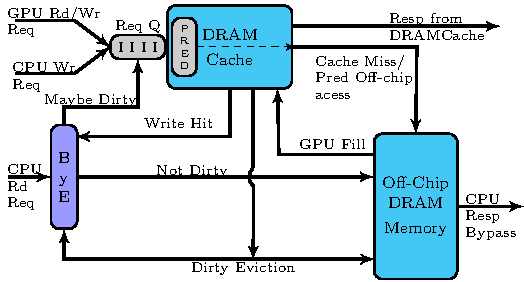
\includegraphics[scale=1.5]{figures/bloom}	
	\caption{Working of \cachename\ with \bypassname}
	\label{fig:bye}
\end{figure}

\par To allow the CPU requests to bypass the DRAM cache, \cachename\ needs to be able to track and lookup dirty lines in the DRAM cache. However, maintaining a list of all dirty lines in the DRAM cache would require prohibitively large storage structures. Thus, \cachename\ uses an approximate tracker called Bypass Enabler (\bypassname). \bypassname\ uses a counting Bloom filter \cite{bloom,counting-bloom} that tracks the dirty lines in the DRAM cache and provides a space efficient way to determine if a given request can be bypassed. The property of a Bloom filter to answer "definitely not in set" allows us to bypass requests correctly i.e., without verifying tags in the set of the DRAM cache. 
On a write request when a cache line becomes dirty in the DRAM cache, the address is hashed into \bypassname\ and the corresponding counters are incremented. When a dirty line is evicted from the DRAM cache, \bypassname\ attempts to remove the entry from the Bloom filter by decrementing the corresponding locations 
\footnote{Counting bloom filters use saturating counters. If counter saturates, decrementing it can lead to false-negatives (dirty lines predicted as clean lines and wrongly bypassed). Hence in our scheme, saturated counters are never decremented.  While this may increase the false positives (clean lines being predicted as dirty), which only reduces the benefits obtained by \textit{ByE}, it does not affect functional correctness. In our implementation we observe that on an average just 2\% of the 2-bit counters in the Bloom-filter saturate out of the 512K counters.}.
\par \bypassname\ bypasses CPU requests only when the GPU cores are executing the kernel. For this, all CPU read requests lookup into \bypassname\ as shown in Figure \ref{fig:bye}. If the Bloom filter search returns a  negative result, then the address is guaranteed to be not dirty in the DRAM cache. Thus, the request can safely be bypassed to utilize the off-chip DRAM bandwidth. 
\par All write requests and GPU read requests proceed serially after looking into the cache. \bypassname\ does not bypass any write requests as it would otherwise require a back-invalidation of the cache line, if present in the DRAM cache, which would need a full DRAM cache access.

\subsubsection{Insertion Policy}
\par Further, when the bypassed CPU requests return from the off-chip DRAM access, these requests are directly forwarded to the requester and are not inserted into the cache. 
Firstly, this allows \bypassname\ to ensure that future write requests for the line do not hit in the DRAM cache as increase in dirty lines would lead to reduced bypass efficiency. 
% (we wanted this sentence cuz we dont want the reader to start thinking of reduced hit rates) Firstly, this allows \bypassname mechanism to continue bypassing future read requests for the line by ensuring that the write requests for  line do not hit in the cache causing reduced bypass efficiency
Secondly, this allows \bypassname\ to reduce some of the bloat caused by a Miss Fill \cite{bear} into the DRAM cache.
Thus, the no-insert policy and the \bypassname\ act as complementary self balancing mechanisms - trading off CPU hit rates in DRAM cache for better access latency at the off-chip DRAM.
\subsubsection{\bypassname\ Hardware Overhead}
\par We find that a small 2-bit counting Bloom filter implemented with two $H_3$ hash functions \cite{h3} and 512K entries per controller is sufficient 
to produce reasonable bypass efficiency with a tolerable misprediction rate. The total overhead for \bypassname\ is 256KB for a 64MB DRAM cache which is less than 0.4\% of the cache size.
\par Thus, \bypassname\ is designed to improve performance by achieving a better bandwidth balance between the DRAM cache and the off-chip main memory.

%-----------------------------------------------------------%

\subsection{Heterogeneity-Aware Spatial Occupancy Control} \label{mechanism-chaining}
\textbf{Objective:} Allow GPU to better use DRAM cache Bandwidth
\subsubsection{Premise}
The schemes proposed in the previous two subsections, \prioname\ and \bypassname, attempt to improve the latency of CPU requests. The mechanism described in this section details \cachename's approach to improve the utilization of the DRAM cache for GPU requests, in order to exploit the higher bandwidth provided by it. 
\par First, we make the following observations and inferences: 

\begin{enumerate}[label=(\roman*)]
	\item The working sets of CPU applications tend to be limited to few tens of MBs due to the limited amount of MLP that can be exploited by the CPUs. Thus, providing larger than certain share of cache leads to no further improvements in hit rates and IPC for CPU. Nevertheless, the CPU can still gain from some share of the DRAM cache due to reduced latency of access.
	\item Further as CPU applications are latency sensitive, the DRAM cache hit latency for CPU requests should not be unduly stretched.
	\item For the GPU to be able to better utilize the DRAM cache bandwidth, the hit rates for GPU workloads should be large enough that the GPU does not have to frequently use the relatively constricted off-chip DRAM buses.	
	\item Given that GPU can exploit much higher MLP using several thousands of threads, the relatively small GPU L2 cache provides limited filtering of traffic and has significantly high miss rates while on the other hand CPUs have sufficiently sized L2 cache sizes to be able to retain blocks longer before re-requesting a block.	
	\item As noted in Section \ref{motivation}, GPUs can trade access latencies for higher hit rates. Thus, providing associativity for GPU request to improve the hit rate would be beneficial.
\end{enumerate}

\par The above observations lead to the following conflicting requirements. It is important to ensure that the CPU requests have certain share (minimum occupancy) in the DRAM cache to ensure the benefits of lower latency while to effectively use the larger share of DRAM cache for GPU requests, it may be required to increase  associativity of the DRAM cache. However such an associativity should not unduly increase the hit latency for CPU requests. 
\par To accomplish the above goals, \cachename\ uses a \chaining\ scheme which introduces (pseudo) associativity mainly for GPU requests, while ensuring a certain minimum occupancy for CPU lines.
\subsubsection{Mechanism Overview}
\par The proposed \chaining\ scheme uses a linear probing \cite{knuth-linear-probing} like technique, inspired by the collision resolution mechanism of a hash map, as shown in Figure \ref{fig:chaining-concept}.
To ensure minimum occupancy for CPU requests, \chaining\ maintains a low-threshold value (\textit{$l_{cpu}$}) and when the occupancy of CPU lines
\footnote{As mentioned earlier we classify a data as CPU data or GPU data based on whose request last accessed the data in the DRAM cache. An alternate equally feasible design point is to classify the data as CPU or GPU data based on which request brought the data into DRAM cache although the CPU and GPU may subsequently access it. In our setup only the CPU core executing the GPGPU application possibly shares data with the GPU and hence we do not expect to see significant difference in the results.} 
reaches this threshold, \chaining\ ensures GPU data does not replace data brought in by CPU. 

\begin{figure}
	\centering
	\def\svgwidth{0.45\linewidth}
	\input{figures/chainings.pdf_tex}
	\caption{Conceptual Working of \chaining\ in \cachename}
	\label{fig:chaining-concept}
\end{figure}

In the other situations, \cachename\ modifies the replacement policy in the DRAM cache depending on the requesting core type. For a GPU request that is evicting another GPU line, \cachename\ looks for a line belonging to a CPU to replace within the same row in the next three consecutive locations,
i.e., if $B$ is the original cache block, then the blocks considered for insertions are $(B+1)\%N_s$,$(B+2)\%N_s$, and $(B+3)\%N_s$, where $N_s$ is number of blocks in a DRAM cache row (page). Hence, the inserted block always lies in the same DRAM cache row as the original cache block. Note that for every set, there could be at most 1 chained set, providing a pseudo-associativity of at most 1.  
We refer to this inserted location as the \textit{chained block} and the actual cache block the request mapped to as the \textit{original block}. The location of the \textit{chained block} is then represented as a 2-bit offset and is stored along with the metadata for the original set (see Figure \ref{fig:chain-access}(a)). When a cache block is evicted, if it was a \textit{chained block}, to unchain it (from the \textit{original block}), the offset stored in the reverse chain bits field in the metadata for the \textit{chained block} is used.  
The chain dirty bit field (Figure \ref{fig:chain-access}(a)) in the metadata indicates whether the chained location, if any, holds modified data. This is used to optimize the access path for CPU and reduce the adverse effect of a double set lookup for latency sensitive CPU requests as shown in Figure \ref{fig:chain-access}(b). \chaining\ relies on the hit/miss predictor to have started an early access to memory. This avoids the second set lookup for CPU if the parallel memory (PAM) access has returned and the chained block is clean. 


\begin{figure}[htb]
	\centering
	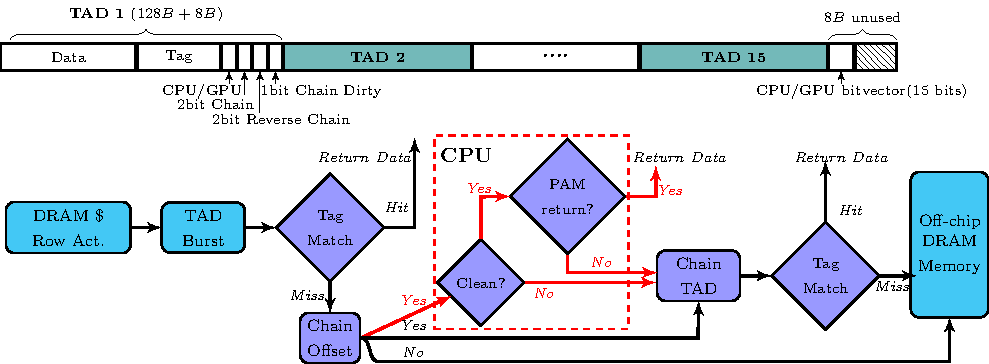
\includegraphics[scale=0.96]{figures/chaining}
	\caption{\cachename\ Row Organization and Access Path of a Request for \chaining}	
	\label{fig:chain-access}
\end{figure}

Additionally, each tag also stores 1 bit information about the owner of the block (CPU or GPU). This bit is used to make quick replacement decisions locally. The additional metadata required for \chaining\ is only 6 bits which can easily be accommodated in the existing 8 byte metadata. Lastly, the unused 8 byte (at the end of each row(page)) is used to store ownership information of each block in the row (15 bits). This information is used to make the \chaining\ replacement decision.


\par As explained earlier, when the \textit{$l_{cpu}$} threshold is reached, GPU lines are not allowed to evict CPU blocks and such GPU requests contending to evict a CPU line are forced to chain to another block belonging to a GPU and evicting that instead, thus maintaining the \textit{$l_{cpu}$} occupancy for CPU. In the very rare case that a GPU block is not found within the 3 consecutive locations the request is not inserted into the cache.

\begin{table}[htb]
	\centering
	\begin{tabular}{|c|c|c|c|c|}
\hline
\multirow{2}{*}{\begin{tabular}[c]{@{}l@{}}Threshold \\ Reached?\end{tabular}} & \multirow{2}{*}{\begin{tabular}[c]{@{}l@{}}Original\\ Set\end{tabular}} & \multirow{2}{*}{\begin{tabular}[c]{@{}l@{}}Not \\ Chained\end{tabular}} & \multicolumn{2}{c|}{Chained Set}                                                                                         \\ \cline{4-5} 
                                                                               &                                                                         &                                                                         & CPU                                                        & GPU                                                        \\ \hline
\multirow{2}{*}{No}                                                             & CPU                                                                     & \begin{tabular}[c]{@{}l@{}}replace\\ original\end{tabular}              & \begin{tabular}[c]{@{}l@{}}replace\\ chained\end{tabular}  & \begin{tabular}[c]{@{}l@{}}replace\\ original\end{tabular} \\ \cline{2-5} 
                                                                               & GPU                                                                     & \begin{tabular}[c]{@{}l@{}}Chain to\\ nearest \\ CPU set\end{tabular}   & \begin{tabular}[c]{@{}l@{}}replace\\ chained\end{tabular}  & \begin{tabular}[c]{@{}l@{}}replace\\ original\end{tabular} \\ \hline
\multirow{2}{*}{Yes}                                                             & CPU                                                                     & \begin{tabular}[c]{@{}l@{}}Chain to\\ nearest\\ GPU Set\end{tabular}    & \begin{tabular}[c]{@{}l@{}}do not\\ insert\end{tabular}    & \begin{tabular}[c]{@{}l@{}}replace\\ chained\end{tabular}  \\ \cline{2-5} 
                                                                               & GPU                                                                     & \begin{tabular}[c]{@{}l@{}}replace\\ original\end{tabular}              & \begin{tabular}[c]{@{}l@{}}replace\\ original\end{tabular} & \begin{tabular}[c]{@{}l@{}}replace\\ original\end{tabular} \\ \hline
\end{tabular}
	\caption{\chaining\ Mechanisms GPU Fill Request Insertion Policy}
	\label{chaining-replacement}
\end{table}

\subsubsection{Insertion Policy}
\par We now summarize the insertion policy used by \chaining\ mechanism in \cachename. 
\par For all CPU fill (insertion) requests, the data is always inserted in the original block, and the victim block is evicted, removing chaining, if any, using the reverse chain bit. 
\par The memory controller maintains a running GPU occupancy counter for each row in the DRAM cache. This information is accommodated in the unused bits at the end of the row in the DRAM cache and can be cached in SRAM structures for fast lookups. Using this current occupancy counter the controller decides the fill policy for the GPU fill request. \cachename\ checks whether the threshold reached is determined by comparing the current GPU occupancy with the set \textit{$l_{cpu}$} threshold value as : $O_{gpu}\le(1-l_{cpu})$ where $O_{gpu}$ is the current GPU occupancy in the DRAM cache row. For a GPU fill request, if the low threshold mark for CPU occupancy is not reached, then the \chaining\ scheme replaces a CPU location, either from the original location or from the chained location, as indicated in row 1 of Table \ref{chaining-replacement}. For a GPU fill request, if the original location belongs to GPU and does not have a chained location, then block is inserted in one of the nearest CPU block [$(B+1)\%N_s$ or $(B+2)\%N_s$ or $(B+3)\%N_s$]. If such a nearest CPU block is not found, the request is inserted into original block itself. If the original location is chained, then the scheme replaces the chained location, if that belongs to CPU or the original location itself, as indicated in row 2 of Table \ref{chaining-replacement}. When the CPU occupancy has hit low threshold, then a GPU fill request replaces the original location if it belongs to GPU (row 4 in Table \ref{chaining-replacement}). If the original location belongs to CPU and does not have a chained block, then the GPU request is chained to the next nearest GPU location. If the original location is chained, but the chained location belongs to GPU, then the fill request replaces that. Otherwise, the fill request is not inserted in the DRAM cache (see row 3 in Table \ref{chaining-replacement}). Thus the \chaining\ scheme ensures, as far as possible, the CPU requests can find the data in the original location, while the GPU requests attempt to exploit pseudo-associativity for increased cache occupancy. In all cases (for both GPU and CPU requests) the access is satisfied with at most 2 tag matches, either in original location or in the chained location (identified by the chain bits). 

\par In essence, \cachename\ uses this \chaining\ mechanism to force occupancy control in the DRAM cache. \chaining\ is able to 
\begin{enumerate}[label=(\roman*)]
	\item ensure a minimum occupancy for the CPU lines while effectively allowing the GPU to occupy the rest of the DRAM cache by providing pseudo-associativity.
	\item remain as a direct mapped cache for majority of the CPU requests.
	\item avoid forcing eviction of hot GPU lines while also avoiding storing of dead lines in the cache.
\end{enumerate}

\subsubsection{\chaining\ Hardware Overhead}
This occupancy control mechanism does not incur any additional storage and uses the unused space in the DRAM cache rows. Once the GPU finishes kernel execution \cachename\ returns to a direct mapped cache as the CPU lines inserted into the DRAM cache occupy \textit{chained blocks} thereby unlinking chains. 

\section{Summary}
In this chapter, we presented the \cachename\ organization and mechanisms. We first showed the conscientious design decisions made and substantiated them with experiments of DRAM cache for IHS architecture. We then detail the principles and working of the three \cachename\ mechanisms - \prioname, \bypassname\ and \chaining. For each of the mechanisms, we describe the issues they try to address, describe their working in detail and the hardware overheads incurred. \cachename\ mechanisms are heterogeneity-aware, lightweight (incurring minimal or no hardware overhead) and can dynamically adapt to the inherent disparity of demands in an IHS architecture.


\chapter{Simulation Infrastructure} \label{chap:simulator}
In this chapter, we articulate the simulator setup and enhancements done to simulate the IHS architecture with the shared stacked DRAM cache. We then outline the experimental methodology, benchmarks comprising of composite heterogeneous workloads used in our evaluation and the parameters used to report system performance in our evaluation.

\section{The gem5-gpu Simulator} \label{gem5-gpu-simulator}
The gem5-gpu \cite{gem5-gpu} is a heterogeneous cycle accurate CPU-GPU simulator used to simulate a hybrid system with both CPU and GPU types of cores. It integrates gem5 \cite{gem5} for the multi-core CPU simulation and gpgpu-sim \cite{gpgpu-sim} for simulating the compute units of a general purpose GPU with a flexible and configurable memory hierarchy using gem5's Ruby memory system \cite{gems}. It can model a system with multi-core CPUs and a discrete GPU with a "split" memory hierarchy or an integrated heterogeneous system with tightly coupled CPU and GPU cores with a "shared" cache coherent interconnect. We refer to the gem5-gpu from here on running an IHS architecture with a shared virtual and physical address spaces as described in Chapter \ref{chap:introduction}. The gem5-gpu can run unmodified operating system and application binaries. The simulator is also performance validated against hardware and is completely open source \cite{gem5-gpu}. For our evaluation we run gem5-gpu in System Call emulation mode with the base operating system performing the CUDA driver emulation.

\subsection{Addition of Shared 3D Die-Stacked DRAM cache}
The Ruby cache and memory hierarchy in gem5-gpu is authored using the domain specific language SLICC (Specification Language for Implementing Cache Coherence) \cite{gems}. SLICC allows the definition of cache levels and behaviour of the coherence protocol. The directory controller is the memory side coherence engine and participates in the coherence protocol. These directory controllers have message queues to send and receive memory requests from the DRAM Controllers. The DRAM controllers are responsible for the operation of the DRAM devices. These DRAM controllers queue requests and orchestrate memory access scheduling to the DRAM according to the type of memory device (e.g., DDR, LPDDR, GDDR, HMC etc). To study the interference of CPU and GPU traffic we model the DRAM cache as the first shared level of cache between the heterogeneous CPUs and GPUs while the L2 SRAM caches are shared between homogeneous CPU cores and GPU cores. We modified the IHS architecture to include a shared split L2 cache shared across multi-core CPUs instead of the default per CPU private L2 cache. For this we modified the existing VI\_Hammer coherence protocol \cite{gem5-gpu} to simulate the shared L2 Cache.
\begin{figure}[!htb]
	\centering
	\def\svgwidth{\columnwidth}
	\input{figures/simulator-memory.pdf_tex}
	\caption{Memory Hierarchy as Modelled in Simulator}
	\label{fig:simulator-memory}
\end{figure}

\par The DRAM cache we evaluate here is a memory-side \cite{skylake,mainak-hpca} shared cache between the 2 split cache hierarchies of CPUs and GPUs. A memory-side caches are ones that are outside the coherence domain as shown in Figure \ref{fig:simulator-memory}. They are logically just in front of the memory and serve to increase the memory's effective bandwidth and reduce the average latency of memory accesses. It does not introduce any new states to the directory in the coherence protocol i.e., there is no state called dirty in DRAM cache, or there is no need to snoop it separately and a single memory state is enough to serve data from it. Further, access to memory is interleaved across multiple memory controllers. To avoid a biased interleaving due to uniformly strided address patterns, in our simulation we employ a basic {\tt XOR}-based address hashing mechanism. Each memory controller manages a 4GB DDR3 memory device and a 32MB stacked DRAM vault. The stacked DRAM vault caches data from the corresponding 4GB memory device that the controller is responsible for. This setup ensures that there are no cross bus requests between controllers. Since our simulation setup has the limitations of having a 1-to-1 channel mapping between a stacked DRAM vault and a off-chip DRAM channel, our model does not provide sufficient channel level parallelism as is essential in a stacked DRAM device. To circumvent this limitation we increase the number of layers (ranks) to provide higher amount of parallelism in our stacked DRAM. However, the bank capacity is retained as would be in a standard stacked DRAM. The DRAM cache is non-inclusive  \cite{coherence-dramcache} of the L2 caches above it and uses a write no-allocate policy. 

\subsection{DRAM cache Controller Design}
The DRAM cache Controller consists of several constituent components as shown in Figure \ref{fig:dramcache-ctrl}. The highlighted components (gray fill) in the figure correspond to the components that are unique/exclusive to a DRAM cache controller and are not present in a conventional DRAM controller. These include fill queue, MSHR and WriteBuffer.

\begin{figure}[!htb]
	\centering
	\def\svgwidth{\columnwidth}
	\input{figures/dramcache-ctrl.pdf_tex}
	\caption{DRAM cache Controller Components}
	\label{fig:dramcache-ctrl}
\end{figure}

\par DRAM cache controllers similar to conventional off-chip DRAM controllers consists of request queues. Each request in the queue corresponds to the address of a single burst of data from the stacked DRAM device.
In our design, cache lines are stored as a TAD units (tag-and-data) \cite{alloy} and each TAD is divided into 2 bursts, where each burst corresponds to the width of the data bus of the stacked DRAM.
Conventional DRAM controllers enqueue requests into a read or a write queue depending on the type of request. 
However, more subtly unlike conventional DRAM devices, each write request in the DRAM cache entails a tag read and match followed by a write to the data of the TAD unit only if the tag matches (i.e., request is a hit). Thus, both read and write requests in a DRAM cache perform a DRAM read operation. To avoid complicating the model and implementation we choose to hold all write requests, irrespective of hit or miss, in the same write queue. This allows us to apply uniform priority to all write requests as these are not in the critical path.
Our stacked DRAM cache also models a third type of queue called a Fill Queue \cite{dca} which enqueues requests to insert data into the cache when the requests return from main memory. A fill request performs a DRAM write operation only. 

\par We also model MSHR and WriteBuffers with their associated latencies to realize the precise working of caches. An MSHR is allocated on a cache line miss in the DRAM cache and subsequent requests to that cache line are coalesced and added as targets in the MSHR. A single fetch request is sent to memory corresponding to an MSHR. Once the memory request returns, a response with the data is sent for each target within the MSHR before it is deallocated. Subsequently, a fill request is also created to insert the TAD back into the DRAM cache. 
A WriteBuffer is allocated when (a) a dirty cache line is evicted from the DRAM cache, thus requiring a write back to memory (b) a write request misses in the DRAM cache. Since the DRAM cache is designed with a write no-allocate policy, write misses in DRAM cache are directly forwarded to the memory. The WriteBuffer is deallocated when the write to memory returns and an acknowledgement is sent to the requester. 
\par When scheduling a request to the DRAM cache, the control logic first selects a queue. The DRAM cache control logic prioritizes reads over writes as reads are in the critical path. This is done by allowing the write queue to fill up to a certain high threshold (\textit{write\_high\_threshold}) before switching the bus for writes. Switching the bus from read to write or vice versa incurs a delay and hence a minimum number of writes (\textit{min\_writes\_per\_switch}) are performed before switching the bus back to servicing read requests. If the read queue is empty, we avoid starving the writes and prevent the device from being underutilized/idle by allowing the bus to switch to writes if the write queue has a certain minimum number of requests (\textit{write\_low\_threshold}). The DRAM cache control logic considers the fill queue as part of the write queue thresholds and switches to servicing a fill queue request in the write mode, only when a fill queue high threshold is reached (\textit{fill\_high\_threshold}). Once the queue is picked, the DRAM cache scheduler then picks a request to be serviced from the queue according to the scheduling algorithm. The address of the request is decoded according to the  address mapping policy and appropriate address and commands are sent over the bus while respecting the device timings and refresh constraints.
\par To simplify data management and ensure correctness we choose not to implement a backing store for the DRAM cache and instead share the backing store instance of the off-chip DRAM itself.

\subsubsection{Reject-Retry Mechanism} Interactions between the components, for example DRAM cache Controller and off-chip DRAM controller, is implemented as a master-slave port architecture. A master port sends requests while the slave port receives requests and invokes appropriate functions to act on the requests. For example, when the directory controller's memory master port sends a request to the slave port of DRAM cache Controller it enqueues the request in the appropriate queue. Similarly, a slave port sends out responses and the master port receives these responses and performs appropriate action. For example, when the DRAM controller responds to the a read request, the DRAM cache controller clears the corresponding MSHR and sends a response to the requester.
\par However, a cache can be in a blocked state when MSHRs or targets within a MSHR or WriteBuffers are unavailable. At such a time, when a request is received at the DRAM cache slave port but is not able to act on it due to the cache being blocked or read/write queue being full or due to mechanism restrictions as in \prioname, the request is rejected and the reason for the blocking is remembered (i.e., the resource causing the block). When the corresponding resource becomes available, a retry message is sent to the master port from the slave port. Once the master port receives this message, the request is resent. This is called the reject-retry mechanism. This mechanism is independent of the network-on-chip that handles routing, channel partitioning etc.

\subsection{System Configuration} 

\begin{table}[h]
	\centering
	\begin{tabular}{{@{}ll@{}}}
		\toprule
		CPU Core 	& five 4-wide out-of-order x86 cores @2.5 GHz \\
		\midrule
		CPU Caches 	& 32KB 8-way split I/D private L1 Cache, \\ 
		& 1MB 8-way shared split L2 Cache, 128B lines \\
		\midrule
		GPU Core 	& eight Fermi SMs@700MHz, 2x2 GTO warp sched\\
		& upto 32 threadblocks, 64 warps of 32 threads, \\
		& 64K registers, 96KB scratch memory \\
		\midrule
		GPU Caches 	& 64KB 4-way private L1 cache,\\ 
		& 512KB, 16-way assoc L2 Coherent Cache \\
		\midrule
		Stacked     & 2 vaults, HMC\_2500\_x64, 2KB Page \\
		DRAM		& $t_{CL}$-$t_{RCD}$-$t_{RP}$-$t_{RAS}$=9.9ns-10.2ns-7.7ns-21.6ns\\
		& 8 layers/vault, 4 banks/layer\\
		& 64 byte burst size, Peak bandwidth 40GB/s \\
		& Refresh related: $t_{REFI}$=3.9us $t_{RFC}$=59us \\
		\midrule
		Off-chip 	& 2 channels, DDR3\_1600\_x64, 1KB page \\
		DRAM		& $t_{CL}$-$t_{RCD}$-$t_{RP}$-$t_{RAS}$=13.75ns-13.75ns-13.75ns-35ns\\
		& 1 rank/channel, 8 banks/rank\\
		& 64 byte burst size, Peak bandwidth 25GB/s \\
		& Refresh related: $t_{REFI}$=7.8us $t_{RFC}$=260us \\
		
		\bottomrule
	\end{tabular}
	\caption{Configuration of the Simulated System}
	\label{configuration}
\end{table}

The gem5-gpu is configured to run 5 CPU cores (4-wide out-of-order cores, operating at 2.5GHz) with a 32KB private L1 Cache (split I/D), and a 1MB shared L2 Cache (shared across all CPU cores). The IHS also consists of 8 Fermi-like compute units, operating at 700MHz with a private 64KB L1 and 512KB shared L2 cache (shared across all CUs). The details of the IHS configuration are given in Table \ref{configuration}. The private L1 of CUs are non-inclusive of the shared GPU L2 cache and can hold stale data. However, GPU L2 cache is coherent with all levels of the CPU hierarchy. The CPU caches and GPU L2 cache are kept coherent in the simulator. Table \ref{configuration} provides the simulator setup details. 
Our simulator also respects all significant timing and functional parameters for the stacked DRAM cache (including refresh, data bus, request queues, scheduling algorithms, command signalling and clock frequencies) using the DRAMCtrl \cite{dramctrl} model.

\section{Workloads} 
Our goal is to study the performance impact of the large last level shared DRAM cache in IHS architectures. Hence we run multiple applications in parallel on the multi-cores and the GPGPU. Applications having high and medium memory intensive behaviours from SPEC CPU2006 suite \cite{spec2006} were chosen to form a multi-programmed workload that run completely on the CPU. Table \ref{single-cpu-mpki} classifies the CPU benchmarks into low, medium and high memory intensity based on the observed MPKI values as seen at the L2 cache when running alone. We create a multi-programmed workload with 4 SPEC benchmarks each. We use the Rodinia benchmark suite \cite{rodinia} to represent GPU applications that offload kernel computation to a GPU CUs. These Rodinia applications are modified to elide the \textit{memcpy} api calls so as to run with unified virtual and physical address spaces (Rodinia-nocopy). 

\begin{table}[htb]
	\centering
	\begin{tabular}{|l|l|}
		\hline
		Low (MPKI $\leq$ 10)          \hspace{5em}      & astar, cactusADM, gcc, gobmk, hmmer, sphinx3    \\ \hline
		Medium (10 \textless MPKI $\leq$ 20) & bwaves, bzip2, leslie3d, libquantum, milc \\ \hline
		High (MPKI \textgreater 20)            & mcf, soplex       \\ \hline
	\end{tabular}
	\caption{MPKI of CPU Stand-Alone Benchmarks}
	\label{single-cpu-mpki}
\end{table}

\begin{table}[htb]
	\centering
	\begin{tabular}{|l|l|}
		\hline
		Low (MPKI $\leq$ 10)                & hotspot, lud           \\ \hline
		Medium (10 \textless CPI $\leq$ 20) &  kmeans, needle, srad   \\ \hline
		High (CPI \textgreater 20)            & streamcluster, gaussian       \\ \hline
	\end{tabular}
	\caption{MPKI of GPU Stand-Alone Benchmarks}
	\label{single-gpu-mpki}
\end{table}

For the Rodinia-nocopy benchmarks we used \textit{needle}, \textit{k-means}, \textit{gaussian}, \textit{hotspot}, \textit{srad}, \textit{streamcluster} and \textit{lud}. The rest of the programs either could not be compiled for IHS architecture or could not run (results in forward progress deadlock errors in the modified simulator). The Rodinia benchmarks use the fifth CPU core to run the initialization section before offloading the kernel to GPU. Thus, our IHS simulates five CPU cores and eight GPU CUs. Table \ref{single-gpu-mpki} categorizes the Rodinia-nocopy benchmarks into Low, Medium and High based on the observed MPKI values (Instructions here refer to thread instructions) at the L2 cache.


\par Combinations of these SPEC quad-core multi-programmed workloads were coupled with a full Rodinia-nocopy benchmark to create a representative mix of applications \ref{workloads} that would run in an IHS system. These composite workloads embody different levels of total memory intensity produced by the CPU and GPU cores.
\par We also measure the footprint of these workloads in terms of number of unique 128B cache blocks accessed at the DRAM cache. The memory footprints range from 70MB to 650MB for quad-core CPU workloads and from 5.5MB to 135MB for the GPU application. The smaller footprints obligates us to use a smaller stacked DRAM cache capacity to make pertinent observations.

\begin{table}[h]
  \centering
  \begin{tabular}{{|l|l|l|}}
    \hline
    \textbf{Name} & \textbf{Multi-program SPEC2006} & \textbf{Rodinia}\\
    \hline
    Qg1& cactusADM;gcc;bzip2;sphinx3 & needle\\
    \hline
    Qg2 & astar;mcf;gcc;bzip2 & needle\\
    \hline
    Qg3 & gcc;libquantum;leslie3d;bwaves & needle\\
    \hline
    Qg4 & astar;soplex;cactusADM;libquantum & k-means\\
    \hline
    Qg5 & milc;mcf;libquantum;bzip2 & k-means\\
    \hline
    Qg6 & bzip2;gobmk;hmmer;sphinx3 & k-means\\
    \hline
    Qg7 & soplex;milc;cactusADM;libquantum & gaussian\\
    \hline
    Qg8 & milc;libquantum;gobmk;leslie3d & gaussian\\
    \hline
    Qg9 & astar;milc;gcc;leslie3d & hotspot\\
    \hline
    Qg10 & gcc;gobmk;leslie3d;sphinx3 & hotspot\\
    \hline
    Qg11 & astar;cactusADM;libquantum;sphinx3 & srad\\
    \hline
    Qg12 & astar;mcf;gobmk;sphinx3 & streamcluster\\
    \hline
    Qg13 & astar;cactusADM;libquantum;sphinx3 & lud\\
    \hline
  \end{tabular}
  \caption{Composite Heterogeneous Workloads}
  \label{workloads}
\end{table}

\section{Simulation Methodology} \label{simulation-methodology}
We fast-forward the initialization phase of each workloads up until just before the launch of the first kernel of the GPU program. We ensure that each executes at least 2 Billion instructions in fast forward and a total of 20 billion instructions of the IHS workloads is executed on an average in the CPU cores. This is accomplished by adding a pause phase to the Rodinia benchmarks for the duration until the initialization quota of the SPEC programs is complete. The benchmarks were then check-pointed after the above fast forward phase. Subsequent detailed simulations with different configurations were run from this checkpoint.
We then warm the cache until the fastest core completes 250 million instructions. During the warmup phase the GPU program is not executed. Timing simulations were then run for at least 250 million instructions for each CPU core, resulting in a total of more than 1 Billion instructions across all the CPU cores and the kernel is executed on he GPU core using the gpgpu-sim component. As is the norm, when a core finishes its quota of 250 million instructions, it continues to execute until all the cores have completed.
\par As stated earlier, the Rodinia application uses the 5\textsuperscript{th} CPU core and offloads the kernel to the integrated GPU. These applications are modified to execute in a \textit{conditioned loop} such that there is no corruption of data structures in the program. The \textit{conditioned loop} is run infinitely and represents the region of interest (ROI) of the Rodinia benchmark. This region includes sections of CPU activity and GPU offloads in the execution, as is typical of a HSA program which will exhibit an interleave of offloaded region and serial CPU section. However, only the performance statistics for the first execution of the \textit{conditioned loop} in the program are considered. 
This is done as the first loop represents the true run of the GPU kernel. The number of \textit{conditioned loops} executed depends on the length of the simulation and the IPC achieved by the GPU. Also, Subsequent loops can achieve better hit rates in cache due to the data fetched by the earlier loops thus not corroborating with the true performance achieved.
In cases where the ROI is longer than the complete run of the CPU workloads, the statistics for the last completed kernel are used. 

\section{Performance Metrics} \label{perf-metrics}
Our study concerns the performance of the IHS architecture, in which multiple single threaded CPU programs and GPU program are co-run and contend for the shared DRAM cache. 
In such a co-run setup, the progress made by the applications (workloads) is different compared to when running homogeneously (i.e., only ran CPU applications on CPU cores or GPU kernels on GPU cores). Further, the performance impact of the shared DRAM cache is not same on the each of the CPU benchmarks as well as the GPU benchmark. We require to define metrics that combine IPC meaningfully without biasing the system performance to either CPU or GPU cores. Hence, we report a multitude of performance metrics to holistically determine the performance of the IHS processor with the DRAM cache and our optimizations. 
\par We report performance of each processor using the intuitive metric of harmonic mean of IPC for the CPU cores and GPU CUs which is defined as 
{
\begin{equation*}
H\textnormal{-}MEAN_{CPU} = \frac{n_{cpu}}{\sum_{i=1}^{n_{cpu}} \frac{1}{IPC_{i}^{CPU}}} \ and \hspace{0.2cm} H\textnormal{-}MEAN_{GPU} = \frac{n_{gpu}}{\sum_{i=1}^{n_{gpu}} \frac{1}{IPC_{i}^{GPU}}} 
\end{equation*}
}
where $IPC_i^{CPU}$ and $IPC_i^{GPU}$ are the instructions per cycle achieved by the $i^{th}$ CPU core and $i^{th}$ GPU CU respectively and $n_{cpu}$ and $n_{gpu}$ are number respectively the number of CPU cores and GPU cores.
In this work, we report CPU and GPU $H\textnormal{-}MEAN$ (and the improvement in them) independently. This is done to identify the impact of CPU and GPU applications on each other, as well as to understand the impact of the proposed modifications on each of the application type. 

\par To report combined system performance we use 2 metrics; the H-Mean of all IPCs and Weighted Speedup for all IPCs. This is important as we would need to see a fair system performance metric without biasing the metric to either CPU or GPU performance. Thus, we report combined system performance using the combined H-MEAN of IPC all CPU and GPU cores which is defined as,
{
\begin{equation*}
H\textnormal{-}MEAN_{IHS} = \frac{n_{cpu}+ n_{gpu}}{\sum_{i=1}^{n_{cpu}} \frac{1}{IPC_{i}^{CPU}} + \sum_{i=1}^{n_{gpu}} \frac{1}{IPC_{i}^{GPU}}} 
\end{equation*}
}
\par Combined system performance using the weighted speedup metric \cite{weighted-speedup} is defined as,
{
\begin{equation*}
Weighted Speedup = \sum_{i=1}^{n_{cpu}} \frac{IPC_i^{CPU_{IHS}}}{IPC_i^{SP}} + \sum_{i=1}^{n_{gpu}} \frac{IPC_i^{GPU_{IHS}}}{IPC_i^{GPU}}
\end{equation*}
}
where ${IPC_i^{CPU_{IHS}}}$ and $IPC_i^{GPU_{IHS}}$ denote the IPC achieved by the $i^{th}$ CPU core and the $i^{th}$ GPU CU when running in a IHS setup respectively. $IPC_i^{SP}$ denotes the IPC of the $i^{th}$ CPU application running in a single core in a stand alone mode. $IPC_i^{GPU}$ denote the IPC of the $i^{th}$ GPU CU when the GPU application is running in a stand-alone mode across all GPU CUs. 

\section{Summary}
In this chapter, we presented the simulator extensions to the gem5-gpu simulator to model a DRAM cache for an IHS architecture. We described the workloads created to evaluate the proposed design and the simulation methodology. Finally, we define the comprehensive performance metrics used to measure the IHS system performance for the various configurations.


\chapter{\cachename\ Results} \label{chap:results}
In this chapter, we first show the effect of CPU and GPU sharing a memory subsystem in an IHS architecture. As shown in section \ref{motivation}, addition of a naive DRAMCache does has a limited performance improvement on the CPU and GPU in the IHS architecture. We then evaluate the results of the proposed \cachename\ mechanisms discussed in chapter \ref{chap:hashcache} and show that \cachename\ is able to improve the performance of IHS. We also compare \cachename\ approach against some of the related works. Further, we show that \cachename\ solution is robust and scales well by performing sensitivity study for the various components.

\section{\cachename\ Mechanisms}
In this section, we present the performance of the different \cachename\ mechanisms (\prioname, \bypassname\ and \chaining) and some combinations of them. We examine the impact of these mechanisms on CPUs, GPUs and the performance of the IHS system as a whole. Figure \ref{results-speedup} (a) and (b) presents the performance improvement in terms of Harmonic Mean of IPC, for CPU and GPU respectively, normalized to the baseline without a DRAMCache. We report the performance improvement due to the introduction of DRAMCache (Naive),  and then the different HASHCache mechanisms  and their combinations.

\begin{figure}[htb]
	\centering
	\includegraphics{graphs/results-cpu}
	\includegraphics{graphs/results-gpu}
	\caption{Speedups obtained by adding a stacked DRAMCache for (a) CPU (b) GPU}
	\label{results-speedup}
\end{figure}
\subsection{PrIS DRAMCache scheduling}
Prioritizing CPU requests with our \prioname\ scheduler at the DRAMCache controller leads to considerable performance benefits for the CPU. By using \prioname, the average access latency of the DRAMCache for CPU requests reduces by an average of 15.3\% and upto 48.9\% over a naive DRAMCache (presentation of detailed data is omitted due to space constraints). Hence, \prioname\ is able to improve the performance of the CPU by an average of 35\% over a naive DRAMCache. However, on the flip side giving aggressive priority to all CPU requests reduces the performance of GPU by 10\% despite the GPU being able to tolerate larger memory access latencies. For some of the benchmarks like Qg3, Qg10, Qg11 and Qg12 the high priority given to CPU requests by \prioname\ impacts the GPU, causing the GPU performance to reduce marginally below the baseline IHS architecture without a DRAMCache. Note however that, in these workloads, the introduction of DRAM cache (naive) itself improves performance only marginally. Our mechanisms (\bypassname and \chaining) further aim to reduce this performance drop for the GPU by ensuring (a) there are fewer CPU requests in the DRAMCache queues (b) GPU requests, despite being deprioritized at DRAMCache, have a better hit rate in the DRAMCache and avoid accessing the off-chip DRAM.
\subsection{ByE for Temporal bypass}
\bypassname\ attempts to achieve improved performance by directing some requests to be served from the off-chip DRAM, thus achieving improved resource utilization and bandwidth balance in the process. \bypassname\ alone achieves 12\% improvement in CPU performance and a 3\% improvement in GPU performance. 
\par The CPU performance improvements are primarily due to bypassed requests facing reduced queuing delays at DRAM. Figure \ref{results-bloom} shows the percent reduction in total memory access latency for CPU read requests achieved by \bypassname\ over an already aggressive naive DRAMCache which employs a hit/miss predictor for CPU requests (primary y-axis). The total memory access latency for CPU read requests reduces by an average of 28\%. The already high hit rates for GPU in the DRAMCache coupled with the no-fill policy for bypassed CPU requests ensures fewer GPU requests at the off-chip DRAM which leads to lesser congestion. Figure \ref{results-bloom} also shows the percentage of incoming read requests bypassed by \bypassname, on the secondary y axis. 
\bypassname\ is able to bypass on an average about 37\% of incoming read requests. On an average 23\% read requests are to dirty lines in the cache which cannot be bypassed.  The remaining 40\% are false positives in our Bloom filter implementation which could have bypassed the DRAMCache. We discuss more on a sensitive study of Bloom filter later in this section. Further, the reduced set contention and lesser number of CPU requests in DRAMCache queues reduces congestion for GPU, which in turn leads to small performance benefits for the GPU as well improving the Harmonic Mean of GPU IPC by 3\% over naive DRAMCache.

\begin{figure}[!htb]
    \centering
    \includegraphics{graphs/results-bypass}
    \caption{Total MemAccLat reduction with \bypassname\ and \% of bypassed read requests for CPU requests}
    \label{results-bloom}
\end{figure}

\par Combining \prioname\ with \bypassname\ allows for the non-bypassed CPU requests at the DRAMCache to be served with a higher priority and hence reducing the queuing delays. \bypassname+\prioname\ performs better than just \prioname\ by 10\% for CPU and 7\% for GPU. Overall \bypassname+\prioname\ achieves 48.5\% improvement in CPU performance over a naive DRAMCache while degrading GPU performance by just 3\%.

\par The somewhat high false positive ratio in our bypass mechanism is due to the large number of dirty blocks in the DRAMCache and the relatively small size of the Bloom filter.  We also experimented with 3 hash-functions while also optimally increasing the array capacity to 312KB (20\% larger) to reduce aliasing and increase the efficacy of bypass. The performance of CPU and GPU using the larger bloom filter (in terms of Harmonic Mean of IPC) normalized to the original bloom filter size is shown in figure \ref{large-bloom}. We observe that the CPU performance improves only by 2.1\% on an average while the GPU remains largely unaffected.

\begin{figure}[htb]
	\centering
	\includegraphics{graphs/results-large-bloom}
	\caption{Performance with a larger bloom filter}
	\label{large-bloom}
\end{figure}

\subsection{Chaining for Spatial Occupancy Control}
As discussed in \ref{mechanism-chaining}, \chaining\ mechanism improves hit rates for GPU while guaranteeing some occupancy for the CPU in the DRAMCache. We empirically determine a suitable low occupancy threshold of the CPU (\textit{$l_{cpu}$}) to be 20\% for all our workloads. Chaining alone performs no better than a naive cache as the queuing latencies overwhelm any improvements in hit rates. However, when chaining is coupled with \prioname, the increased hit rates reduces the performance drop caused by \prioname\ for the GPU from 10\% to 5.2\% (i.e 4.8\% performance improvement over \prioname). For the CPU, guaranteed occupancy in the DRAMCache and the secondary effect of lower congestion at off-chip DRAM allows CPU requests to be serviced with lower delays. This improves performance of CPU by 7\%, over only \prioname.
\par Overall \chaining+\prioname\ improves CPU performance by 44.7\% while degrading GPU performance by merely 7\% over a naive DRAMCache.
% %This improves overall system throughput by a significant 37.7\% over a un-optimized DRAMCache.


\subsection{System Performance with \cachename}
\begin{figure}[!htb]
	\centering
	\includegraphics{graphs/results-system}
	\includegraphics{graphs/results-weighted-speedup}
	\caption{(a)Harmonic Mean (b)Weighted Speedup of IHS with \cachename}
	\label{results-system}
\end{figure}
We now holistically examine the performance improvements due to the introduction of our \cachename\ mechanisms, in  CPU and GPU cores together. From Figure \ref{results-speedup} we observe that, adding a naive DRAMCache can achieve an average of 42\% and 24\% improvement in CPU and GPU cores respectively. Whereas, \cachename\ achieves significant speedups of (205\%,17.5\%) and (211\%,20.4\%) for (CPU,GPU) using Heterogeneity-aware mechanisms of \bypassname\ and \chaining\ respectively. This comes within 16\% and 13\% of the ideal no interference performance for the GPU (final gray bar in Figure 8(b)) and within 81\% and 76\% of the ideal no interference performance for the CPU (final gray bar in Figure 8(b)) for each of the schemes. Further, for memory intensive combination of CPU and GPU workloads like Qg7 and Qg8 which see significant degradation in performance of both processors due to interference, adding a DRAMCache can improve performance upto 430\% for CPU and 48\% for GPU over a baseline system with no stacked DRAMCache. In comparison, the naive DRAMCache implementation only brings 55\% and 56\% improvement in the CPU and GPU performance respectively
\par Figure \ref{results-system}(a) plots the performance improvement as a Harmonic mean of IPCs of IHS IPC (combined CPU cores and GPU CUs), normalized to our baseline IHS architecture without a DRAMCache. Overall with simple heterogeneity aware management of the stacked DRAMCache, IHS systems can achieve on an average 200\% (upto 400\%) performance improvement while a naive DRAMCache is able to achieve just 41.8\% improvement.
\par As a comprehensive system metric Figure \ref{results-system}(b) plots the weighted speedup normalized to the baseline of IHS without DRAMCache. Adding a DRAMCache to IHS processors naively achieves an improvement of merely 3\%. In fact for some workloads like Qg3 and Qg11 adding a DRAMCache without careful considerations can lead to negative performance impact. However, our heterogeneity-aware mechanisms are able to achieve on an average of 16\% and 15\%  improvement in performance over a IHS architecture without a DRAMCache. This improvement corresponds to a 12.9\% and 11.5\% improvement for each of the schemes over a carefully designed but heterogeneity unaware DRAMCache for the IHS processors.

\section{Comparison with related work} \label{comparison}
\begin{figure}[!htb]
	\centering
	\includegraphics{graphs/results-comparison-cpu}
	\includegraphics{graphs/results-comparison-gpu}
	\caption{Comparison of \cachename\ against MCC \cite{mostly-clean} and SMS \cite{sms} (a)CPU (b)GPU}
	\label{results-comparison}
\end{figure}

The objectives of \bypassname\ and \prioname\ are similar to the Mostly Clean DRAMCache (MCC) \cite{mostly-clean} and Staged Memory Scheduling (SMS) \cite{sms} respectively. Hence we compare our work with MCC (adapted for IHS architecture) and SMS in Figure \ref{results-comparison} which presents performance of (a)CPU and (b)GPU normalized to a IHS with no DRAMCache. 
Overall, \bypassname\ performs 7.8\% better than MCC in terms of CPU IPC.
This is because when a page (row) is marked as write-through in MCC, all requests to that page are bypassed oblivious of source of the request. The large number of GPU requests to the cache lines in the write-through (clean) pages quickly exhausts the available MSHR entires which leads to the DRAMCache being blocked for subsequent requests. For workloads Qg9, Qg10 and Qg12 the GPU workloads are relatively less intensive and MCC tends to perform slightly better than \bypassname. The GPU performance is comparable for both approaches. \\
The striped bars in Figure \ref{results-comparison} show the performance of the \prioname\ and SMS for (a)CPU and (b)GPU. For SMS implementation, we proportially scale down the total hardware requirements to the same size as that of \prioname\ (128 entries). We observe that \prioname\ performs on-par with SMS for almost all CPU workloads. For workloads like Qg2 and Qg12 SMS performs marginally better than \prioname\ as it is able to better manage CPU inter-application interference using SJF scheduling. However for the GPU, SMS performs 4\% better than \prioname\ due to its batching algorithm that is able to admit row buffer hit requests into the queues which leads to improved row buffer hit rate (9\% better). Our combined mechanism of \prioname+\bypassname\ proposed in this work performs better then each of prior compared schemes for both CPU and GPU.

\section{Sensitivity Study}
\subsection{Larger Capacity DRAMCache}
\begin{figure}[!htb]
	\centering
	\includegraphics{graphs/results-128M-cpu}
	\includegraphics{graphs/results-128M-gpu}
	\caption{Sensitivity Study with 128MB DRAMCache (a)CPU (b)GPU}
	\label{results-128m}
\end{figure}
We conduct a sensitivity study for \cachename\ mechanisms with a larger 128MB stacked DRAMCache. Figure \ref{results-128m} presents the performance of a naive DRAMCache and our mechanisms \bypassname+\prioname\ and \chaining+\prioname\ for the (a)CPU and (b)GPU in terms of H-Mean of IPC normalized to an IHS with no DRAMCache. We observe that the larger naive DRAMCache is able to achieve 54.5\% and 29.8\% improvement for CPU and GPU processors. \cachename\ mechanisms continue to provide an average improvement of 46\% and 39\% for the CPU, on an average, above a heterogeneity unaware DRAMCache and 226\% and 215\% over the baseline IHS. 
In the larger DRAMCache, Chaining+PrIS results in 15.8\% improvement over baseline (10\% decrease over naive), we
expect the scheme to catch up the lost performance (over naive) in benchmarks with larger GPU footprint.


\subsection{Off-chip DRAM with same latency as DRAMCache}

\begin{figure}[!htb]
	\centering
	\includegraphics{graphs/results-ddr3-2133-cpu}
	\includegraphics{graphs/results-ddr3-2133-gpu}
	\caption{Sensitivity Study with DDR3-2133 off-chip DRAM (a)CPU (b)GPU}
	\label{results-2xbw}
\end{figure}

Although we expect the smaller sizes of stacked DRAMs to have lower latency than off-chip DRAMs, commercial stacked DRAM like those in Intel's Knights Landing \cite{xeonphi} have access latencies similar to off-chip DRAMs. Hence, we scale up the off-chip DRAM to DDR3-2133 like device with latencies (13.09ns-13.09ns-13.09ns-33ns) for $t_{CL}$-$t_{RCD}$-$t_{RP}$-$t_{RAS}$. As before, Figure \ref{results-2xbw} presents the performance (H-Mean of IPC) of (a)CPU (b)GPU with a naive DRAMCache and \cachename\ normalized to a IHS system with no DRAMCache. For \prioname+\bypassname, CPU performance impoves by 48\% while reducing merely 3\% of GPU performance. For \prioname+\chaining, CPU performs 47\% better than a naive DRAMCache while decreasing GPU performance by 4.4\%.

\subsection{Higher Bandwidth DRAMCache}

\begin{figure}[!htb]
	\centering
	\includegraphics{graphs/results-2xbw-cpu}
	\includegraphics{graphs/results-2xbw-gpu}
	\caption{Sensitivity Study with 2x Bandwidth for DRAMCache (a)CPU (b)GPU}
	\label{results-ddr3-2133}
\end{figure}

We carry out experiments for \cachename\ with a stacked DRAMCache of 80GB/s. We achieve this by doubling the burst length of the stacked DRAMCache devices. Again, Figure \ref{results-ddr3-2133}  presents the performance of a naive DRAMCache and \cachename\ for (a)CPU and (b)GPU. We observe that our mechanisms scale with increased DRAMCache bandwidth and \bypassname+\prioname\ performs 51\% better and \chaining+\prioname\ performs 47.3\% better than a naive DRAMCache for CPU. GPU performs also improves by 1.9\% and 2.4\% over a naive DRAMCache. Notably for GPU benchmarks like streamcluster and gaussian \chaining+\prioname\ performs better than \bypassname+\prioname.


\section{Related Work} \label{related-work}
State-of-the-art stacked DRAM device designs have primarily focused on improving the performance of multi-core architectures. %Principally there have been 2 different approaches for using the stacked DRAM devices. 
In \cite{pom,cameo} the stacked DRAMs are organized as part of memory in view of the large capacities provided by these devices. The designs propose hardware management schemes for swapping hot pages into and out of the stacked DRAM devices.
On the other hand, several designs propose to use the stacked DRAM as transparent hardware managed cache. Sectored caches such as \cite{footprint,unison-cache} allocate large blocks and avoid wastage of bandwidth by intelligently fetching useful blocks only. In Section \ref{design} we have broadly alluded to some of the works of DRAMCache designs and organizations \cite{alloy,atcache,bimodal,loh-hill} that organize DRAMCache at smaller system-sized blocks (64B or 128B).
%There are a number of designs around organizing DRAMCache at smaller system-sized blocks (64B or 128B) or an intermediate block size (512B, 1024B or 2048B). 
These designs intelligently manage metadata and tag lookup serialization by using approximate hardware structures. \cachename\ extends and adapts the simplicity and effectiveness of the Alloy Cache organization for IHS architecture after carefully considering the implications of each design decision on performance. 
While these works have focused on improving multi-core CPU performance, our work shows that there exists a large potential for performance improvements by using stacked DRAMCache in a IHS architecture. 
\par Orthogonal to these efforts, there have also been proposals such as \cite{software-dram} to expose the stacked DRAM to the applications and/or system software by providing special allocation calls or using intelligent page management algorithms in system software to place hot data in the high bandwidth memory. Besides these designs incurring the obvious overheads of software modification to improve performance, they also require a good understanding of program behavior and IHS architecture knowledge.
\par Recently, researchers have pointed out the need to utilize all the available bandwidth from both on-chip and off-chip DRAM devices due to comparable access latencies \cite{mostly-clean,mainak-hpca,bear,micro-refresh,mostly-clean-direct} to extract best performance and improve resource utilization. However, \cachename\ uses the ingrained disparity in the requests rates and their implication on performance of each core to optimize bandwidth balance in a heterogeneity aware manner. 
\par Complementary to our own work, there have been efforts to improve performance of IHS systems in \cite{gpu-concurrency} by throttling the GPU cores using intelligent warp scheduling and avoiding congestion in the network-on-chip (NoC) \cite{interconnect}. To manage shared on-chip SRAM caches, Lee et al. \cite{tap} propose heterogeneity aware schemes that are built on top of UCP and RRIP schemes for managing shared  resources. While our chaining mechanism is in line to this to ensure minimum occupancy for CPU requests, it also goes beyond by introducing pseudo-associativity and improving hit-rates (specifically for GPU requests). Mekkat et al. \cite{helm} further propose shared SRAM cache management for IHS workloads that uses runtime metrics, like cache sensitivity of each workload, to allocate cache capacities. Despite larger capacities, DRAMCaches have higher latencies and hence will not be able to adapt quickly enough to SRAM occupancy management schemes proposed in these works.
\par Zhan et al. \cite{oscar} propose improving performance of IHS architectures by replacing on-chip SRAM caches with slightly larger STT-SRAM caches that are non-volatile but have asymmetric read/write energy and latencies. They focus on NoC related optimizations through NoC reordering/batching schemes and differential CPU/GPU, read/write prioritization. The NoC optimizations are orthogonal and can be supplemented to the ideas proposed in this work. The performance improvement due to introduction of STT-RAM in IHS architectures is equivalent to that observed in our naive DRAM scheme.
%\par Lastly, Ausavarungnirun et al., \cite{sms} propose staged memory scheduling for main memory (DRAM) in IHS processors and is similar in spirit to our \prioname, which is applied at the DRAMCache. \prioname uses a relatively simpler approach for prioritizing CPU requests while ensuring that GPU request are not significantly starved. 
\par The authors in \cite{qos-aware} propose a QoS aware memory scheduler to avoid the GPU from missing a frame rendering deadline. However, in our IHS architecture the GPU is used to accelerate general purpose code and hence \prioname\ does not consider such deadlines for the memory controller.
% should we mention HSC coherence paper or sNeha agarwal papers?
\chapter{Conclusions} \label{chap:conclusion}
In this chapter, we summarize the \cachename\ solution and discuss potential avenues for future work.
\section{Summary}
Stacked DRAMCaches require careful design to be able to improve performance of workloads. There are several conflicting factors that require careful consideration and trade-offs. This is compounded by the fact that in IHS architectures the processors themselves are  heterogeneous and have disparate requirements from the DRAMCache i.e., latency for CPUs vs throughput for GPUs.
\par In this work, first we demonstrated that current memory hierarchy requires to be revisited for IHS architectures to be able to perform upto capacity. We presented a case for performance improvement of an IHS processors by addition of a stacked DRAMCache. 
We quantify the effects of interference due to co-running on each processor and show that the heterogeneity adversely effects CPU performance as compared to the GPU. 
Consequently, we carefully design an effective DRAMCache organization for IHS processors by evaluating the design space of DRAMCaches.
Further, we propose three simple and effective heterogeneity-aware techniques --- a heterogeneity-aware DRAMCache scheduler (\prioname), a heterogeneity-aware temporal bypass (\bypassname) and a heterogeneity-aware spatial occupancy control (\chaining) scheme to improve the performance IHS architectures.
\par We develop the simulation modules and infrastructure to simulate an IHS architecture with a DRAMCache. We use a suitable methodology for detailed simulation of \cachename and adapt metrics to measure performance of the proposed system. Using this experimental setup we show that 
\cachename\ achieves significant improvement of 100\% in overall system performance on an average over a baseline system with no DRAMCache and 41\% over a heterogeneity unaware DRAMCache. 
We also show that \cachename\ mechanisms scale very well with stacked DRAMs of larger capacity, higher bandwidth and even with access latencies of off-chip DRAMs.
This work, thus shows that there are significant benefits of using a stacked DRAMCache for IHS processors, far exceeding the usefulness of such devices in homogeneous GPUs and multi-core CPU systems.

\section{Future Work}
An interesting direction for future work would be to explore differential granularity caching for IHS architectures in the stacked DRAMCache for CPU and GPU cores since GPU benchmarks have good spatial locality. Larger blocks with critical sub block first and early restart \cite{dram-book} consequently might prove beneficial as well. Prefetching GPU lines without overly polluting the cache would be another approach to serve GPU lines out of the DRAMCache thus better utilizing the large stacked DRAM bandwidth. However, such techniques need to be mindful that both the memory and cache are slower DRAM devices. 
\par Exploring ways of combining \prioname, \chaining\ and \bypassname\ as a unified technique is likely to improve performance. However, as the objectives of Chaining and ByE are somewhat conflicting, this requires careful consideration of replacement (fill) policies in the DRAMCache.
\par It would also be interesting explore the performance of \cachename\ mechanisms in Collaborative Heterogeneous Applications benchmarks (Chai) \cite{chai} where the CPU and GPU are used concurrently by the same application. DRAMCache management schemes using program hints about the collaboration patterns such as data partitioning, fine or coarse grain task partitioning would also be a interesting future work.
\par Since the IHS architectures use a shared virtual and physical address space, using TLBs to make the DRAMCache tagless might be a practical solution. However this requires careful consideration of the TLB reach and page walker state machine in IHS architectures.




\bibtitle{References}
\bibliography{references}
\bibliographystyle{plain}
\end{document}
